\chapter{Structural Bioinformatics of PVC Proteins}\label{structbioinfo}

\epigraph{\emph{``It is very easy to answer many of these fundamental biological questions; you just look at the thing!''}}{\textit{Richard P. Feynman}}

\section{Introduction}

As large multi-partite biological complexes, there are far too many proteins involved in the biology of PVCs to study them all, in detail, experimentally within a single project. However, due to the increasing availability of high performance computing resources, it is possible to study all the genes and proteins, to some extent and to reasonable confidence, using bioinformatics approaches, such as homology modelling, which is becoming increasingly popular as the rate of high quality genome sequences vastly outstrips the rate of experimental protein structure resolution \citep{Rodriguez1998}. This chapter attempts to glean as many clues as possible about structure and function of the proteins involved in construction of PVCs, by `brute force', with the application of techniques which have not been attempted to date.

Since there are numerous PVC operons that have been identified, and each one contains $>$16 proteins, the dataset quickly becomes unmanageable for the experimentalist. A rigorous exploration of the hypothetical structures and functions of the proteins can collapse this dataset somewhat, and reveal subtleties of the structures which are interesting or relevant for further study. 

As the databases for gene function and protein structure are continuously updated and improved, this chapter is also a `revisit' to the now outdated genome annotations that were first put together when the strains were sequenced. By re-running these analyses at various points, new putative functions and homologies may be discovered.

Furthermore, this chapter is intended to `pull double duty' somewhat; to serve both as an exploration of new roles and information regarding PVC proteins, but also as a continued, extended, introduction or `guided tour', to orient the reader with respect to PVC operons, including what is known about each of the individual proteins within the PVCs, in a similar manner to the exploration of related structures in the Introduction. Hopefully, therefore, this chapter will provide the reader with a understanding of the PVCs with regard to what is already known and what has been discovered, on an almost gene-by-gene basis.

\subsection{The sequence identity problem}
Despite progress in the elucidation of many related structures, as shown in \vref{intro}, much is still unclear with regard to PVCs. Many PVC proteins in the existing \Pa{} annotations are listed as `hypothetical proteins' with no useful information - in some cases, this can be the entire operon \citep{Duchaud2003}. The frequent lack of known good homologues from studying the genes through BLAST for instance, and the degree of sequence diversity that can be seen in the PVCs (see \vref{bioinformatics} for a more in-depth discussion), despite producing the same structure, suggested that structural studies might offer additional/better information.

It is now a widely accepted phenomenon that sequence identity cannot always provide sufficient structural understanding on its own, as the evolutionary rules that constrain structures are not exactly the same as those that constrain sequences. Consequently, protein structures are known to evolve slower than the amino acid sequence, and slower still than the nucleotide sequence. In fact, this rate of change has even been quantified, and is estimated to be between three and ten times as slow \citep{Illergard2009}. Moreover, proteins with entirely unrelated sequences can give rise to functionally equivalent proteins, meaning this analogy between proteins would be completely missed through sequence studies alone. Now, of course this does not completely devalue the position of the sequence in determining protein structure and function, however, as \cite{Illergard2009} and \cite{Chothia1986} explain, the relationship between structural similarity (as quantified by Root Mean Square Deviation (RMSD)), and sequence identity is not linear. One of the earliest papers to explore this disconnect defined a so-called `twilight zone' of structural similarity, observing that once sequence identity dropped to around 25\% and below, false positive hits begin to predominate \citep{rost1999twilight}. Just to labor the point a little further, \cite{Holm1996} explain how structures are able to remain much the same, ``even when all sequence memory appears
to have been lost". This means that for proteins whose common ancestors are extremely far back in time, it effectively becomes meaningless to compare the DNA or amino acid sequences, and only the 3D structure matters. The authors summarise this quite nicely with the analogy, 

\begin{displayquote}
``Comparing protein shapes rather than protein sequences is like using a bigger telescope that looks farther into the universe, and thus farther back in time, opening the door to detecting the most remote and most fascinating evolutionary relations."
\end{displayquote}

To make matters worse, even proteins which \emph{do} share significant sequence identity, do not necessarily have the same structure, and therefore may differ in function. A really good example of this is epitomised by the ``Paracelsus challenge". Posed by \cite{Rose1994}, the challenge was to convert one protein's conformation to that of another protein by altering less than 50\% of the sequence. This was achieved first by \cite{Dalal1997} (winning them a \$1,000 wager in the process), and though they did have to change roughly 44\% of the protein and include an additional 7 amino acids for solubility (bringing to mind a somewhat `Ship-of-Theseus' argument), they were able to convert an almost entirely $\beta$-sheet protein in to an entirely $\alpha$-helical one. Subsequently, their effort has been bested by the work of \cite{Alexander2007}, and thoroughly hammers home the message of ``sequence $\neq$ structure". They were able to convert domains from \emph{Streptococcus} G proteins to retain 88\% sequence identity, yet to change their fold structures, all the while keeping their ligand binding activities.

In short, there is no substitute for being able to \emph{see} the tertiary structure and individual folds for each and every protein. This is far from a solved problem however, as it currently requires exhaustive computation and experimental efforts to generate this kind of data. Protein structure simulation has advanced significantly, but is not without its flaws, and of course, the lottery that is protein structure determination via crystallography for example is an incredibly intensive process with a high failure rate. 


Finally, to underscore this idea with some relevant examples, \cite{Leiman2010} observed that ``evolutionary relationships cannot be detected in their [tailed phages] amino acid sequences", but many structural proteins of phage origin share tertiary structure folds. One rationale for this is that given the high turn over rate of phage genomes, their evolution will occur rapidly, and thus they will explore the `chemical space' rapidly also. This is combined with the fact that phages experience a multitude of evolutionary pressures, and being proteinaceous entities only, they have to be particularly `inventive' when it comes to protein structure robustness. A further example from the same paper concerns the structures of the VgrG spike proteins. They are often structurally very well conserved which is usually immediately apparent on visual inspection, and yet, the sequences of certain orthologues may share $<$15\% amino acid similarity, and due to redundancy, even lower nucleotide identity. Table 1 in \cite{Browning2012} underscores this further, using HHPred to identify the same OB-fold VgrG and T4 spike complexes, despite as little as 16\% amino acid similarity in that particular case. This effectively means that to try and study sequences such as these using sequence data alone would be almost indistinguishable from random noise (though it may be possible to consider small numbers of highly conserved/`privileged' sites). \cite{Silverman2012} make the same observation for the tube proteins (Hcp/TssBC and the VgrG spike).

A further complication with purely sequence based studies, for long, multicomponent operons such as the PVCs and other caudate structures, is that it seems synteny and gene copy may also be significant, potentially playing a role in how the assembly is choreographed (phage early versus late proteins for instance). Papers like that of \cite{Sarris2014}, note that while many of the gene products are identifiable between orthologous operons, the gene copy number varies, as does the syntenic arrangement. In the case of the MAC complex discussed in the first chapter, the whole complex isn't even encoded in one location in the genome \citep{Shikuma2014}. 


To summarise, this chapter looks to address this `conservation of structure not sequence' question with regard to the PVCs, with the aim of identifying new roles for proteins for which sequence identity-based studies have failed to produce useful information; and to infer from these structures in such a way as to provide lab-testable hypotheses.

\subsection*{Chapter Aims}

\begin{itemize}
	\item Complete a thorough and sensitive functional annotation of as many PVC proteins as possible.
	\item Generate structural data and compare it to known proteins.
	\item Examine any high quality simulations for physical characteristics of the PVCs.

\end{itemize}

\clearpage

\section{Experimental procedures}
Given the lack of informative annotations from existing genomes available, the first step was a deeper dive in to the orthologies for all the CDSs from 16 PVC operons. Any information that can be obtained which improves on annotations of `hypothetical protein', even if weak, might provide insights which can be used to plan experiments in future.
	 
%    	\subsection{Annotation}\label{annotation}
%    	From a previous project, a number of \Pa{} genomes were sequenced, and a number of existing sequences in NCBI were reassembled and re-annotated along with them for consistency. In all of the work conducted, we utilised the consistent, re-annotated sequences and any given locus tags will correspond to these. Genomes were annotated with a database of existing \Pa{} proteins, utilising Prokka \citep{Seemann2014} (see \vref{methods},  \vref{prokka}).

\subsection{Methods used for probing the structures of PVC proteins}
\subsubsection{Hidden Markov Model Homology Searching}\label{hhresults}
As the Protein DataBank and other databases are frequently updated, Hidden Markov Model searches were run repeatedly throughout the course of the project, usually picking up at least 2 or 3 improved structural annotations, with each new database version. This was performed using $\mathtt{HHsearch}$ from the HHsuite of tools \citep{Remmert2012}, and was queried against the Protein DataBank each time.
	
Hidden Markov Models (``HMMs") are a sensitive way of searching for sequence similarity, that can outperform tools such as BLAST in certain situations. A Markov Model can be thought of as representing each position in the sequence as being one of many different amino acid possibilities, which are weighted according to their likelihood \citep{Eddy2004}. This arises from the fact that not all amino acids are equally likely to appear adjacent to one another - for instance, a stretch of amino acids, all of which can form $\beta$-sheets, are more likely to appear near one another than would an amino acid which contributes to helices, and thus HMMs capture domain information very well. They are especially suited to the task of identifying distant and very variable homologies, in fact, to quote directly from the HHSuite manual: ``HHsearch and HHblits [different algorithm implementations] can detect homologous relationships far beyond the twilight zone, i.e., below 20\% sequence identity. Sequence identity is therefore not an appropriate measure of relatedness anymore".

Individual homologies for different sections of the PVC operons will be discussed in the coming sections. In overall terms, there are 2 loose distributions to the hits. As the histogram in \vref{probhist} shows, of the roughly 350 sequences that were profiled, about half are extremely well matched, with probability scores of approximately 85\% or higher. The probability score from HHSuite is essentially a measure of how good a match is to a query in terms of their likelihoods of being orthologues. It functions similarly to the more common E-Value, but also takes in to consideration the secondary structures of the proteins matched, which is partly why it is able to reliably identify more distant matches than sequence identity alone. Since all the PVCs carry different effector molecules, and they are reasonably well characterised to date, this chapter will focus on the `dark matter' of the structural region of the operons - not to mention, effector biology of the PVCs could be a PhD thesis in itself.

At the outset of this work, in the $\approx$ 350 studied PVC CDSs, 249 of them were annotated as hypothetical proteins. As a result of further probing through HMMs, all loci have garnered a hit/annotation of some sort, though there are still some unreliable hits. The least well profiled genes primarily consist of: PVC14 - a protein inferred to be a tube tape measure protein from the studies of \cite{Rybakova2013}; PVC7 - an unknown protein which does, however, attract consistent annotation in almost all operons to a SIR2 metalloprotein deacetylase \citep{Shore2000}, but with a huge range of hit scores (E-values ranging from +0.00024 to \sn{4.7}{-5}); and to other assorted unique genes which do not mesh with the consistent nomenclature. These include several from the PVClumt operon, which in many ways appears to be a particularly unusual operon, and other unusual genes such as an additional locus in the PVCUnit2 locus of \Plum{} TT01, between the canonical PVC13 and 14. Unsurprisingly, the proteins with the highest confidence hits matched those with the best annotations before the project began, namely the sheath proteins and toxin enzymes. That said, many of the initial annotations for the tube proteins provided little more information than that they shared similarity with phage tail ``major" and ``minor" proteins. Through HMM searching, these annotations have begun to point to more specific matches such as gp19 orthologues and the sheaths of R-type pyocins. Moreover, subtle differences in the `conserved' sheath proteins reveal that not all operon's sheath proteins match the same orthologues.


\begin{figure}[h]
\thisfloatpagestyle{IHA-fancy-style}
\centering
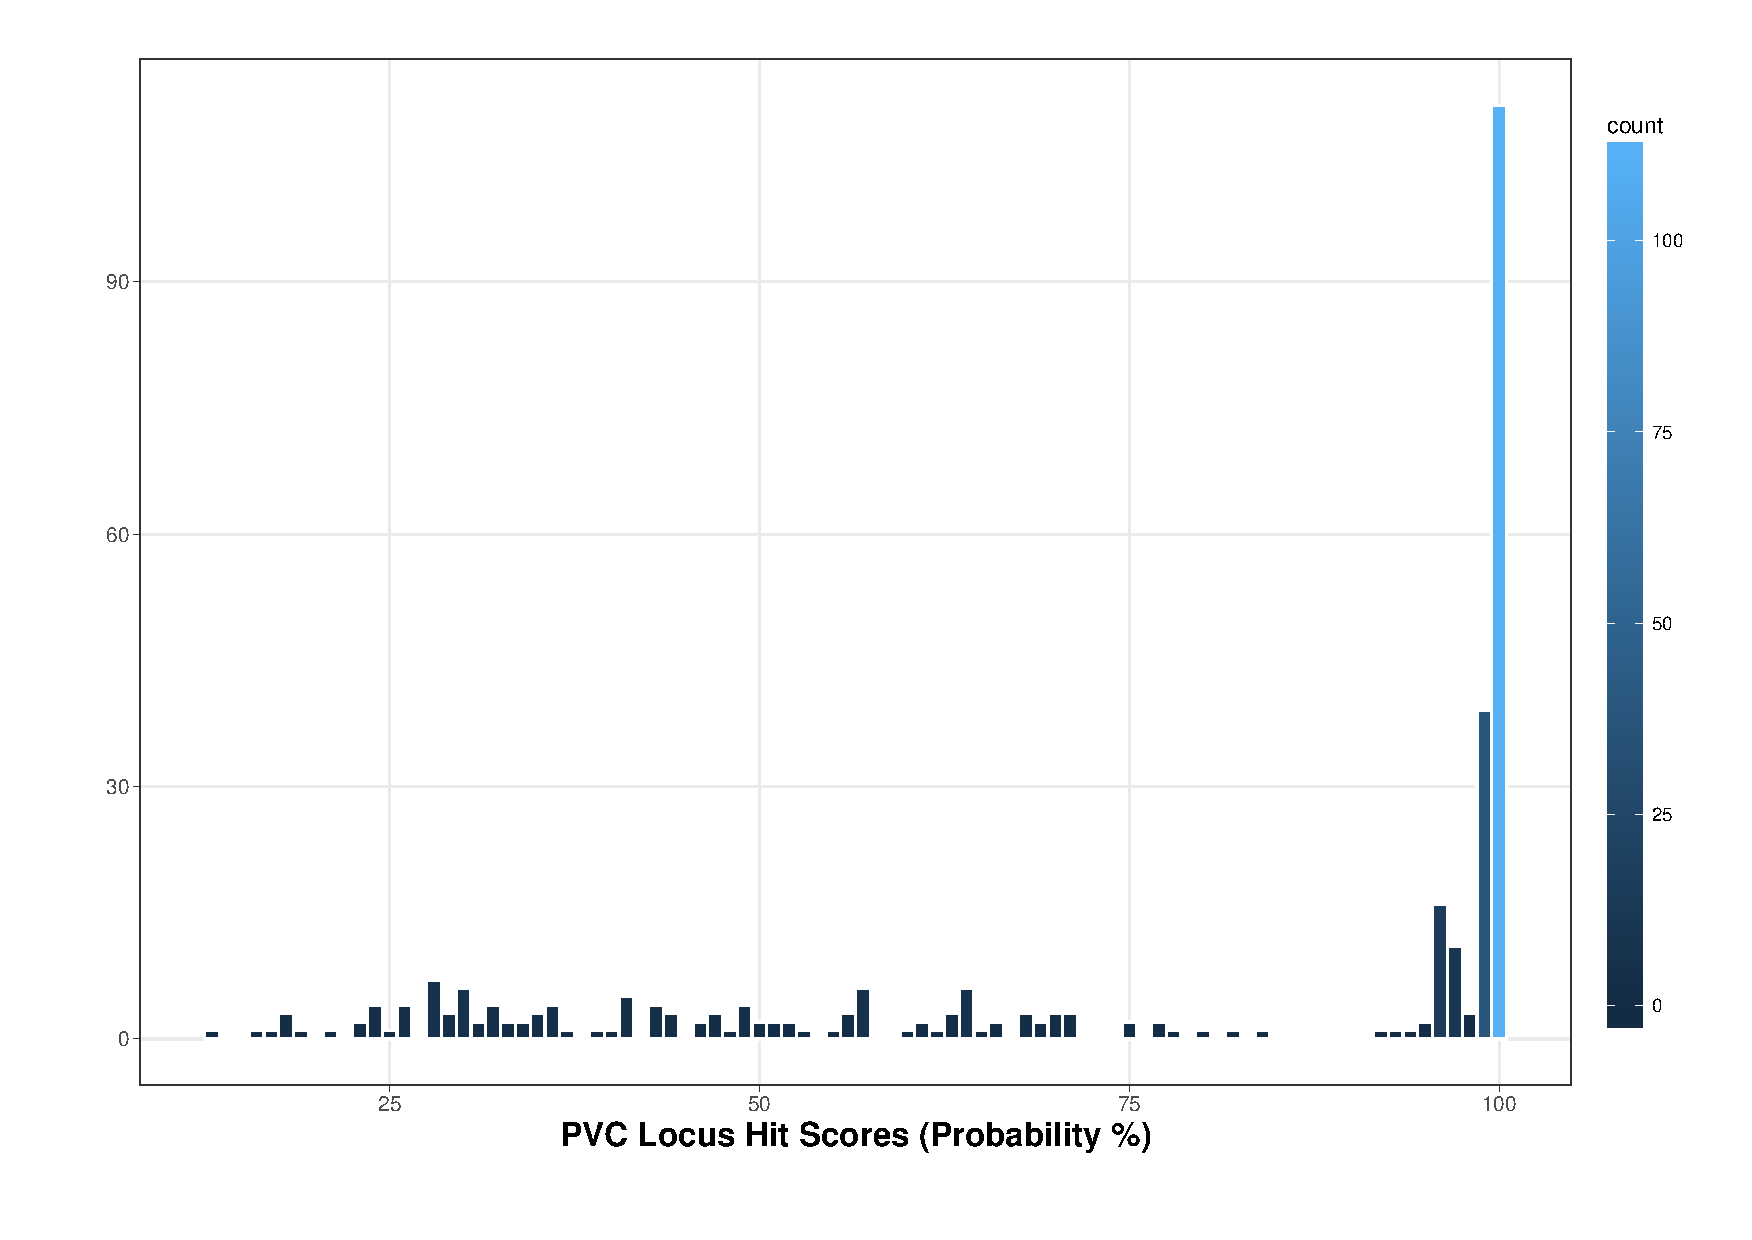
\includegraphics[width=0.9\textwidth]{/Users/joehealey/Documents/Warwick/PhD/Thesis/chapters/chapter3/img/Probabilities.pdf}
	\captionsetup{singlelinecheck=off, justification=justified, font=footnotesize, aboveskip=10pt}
	\caption[HHPred orthologue match scores]{\textsc{\normalsize Distribution of match probabilities for PVC proteins.}\vspace{0.1cm} \newline A histogram of the ``Probability" score for approximately 300 PVC protein sequences. Bars are coloured according to the bin density. Around half of all the proteins are well profiled in this manner, with Probability scores over 80\%. The remaining proteins are distributed widely with a number of examples of proteins which remain with low scores and little to no informative matches.}
	\label{probhist}
\end{figure}


\subsubsection{Homology modelling, threading and structural refinement}
Protein structure modelling was performed using a local installation of the I-Tasser pipeline, on 12 virtual machines \citep{Yang2014, Roy2010, Zhang2008}. I-Tasser was chosen as it generates full length models (whereas some tools only produce models for regions adequately represented by sequence homology), and because it takes a somewhat hybrid approach to modelling, using threading templates, but also \emph{ab initio} molecular dynamics steps for modelling regions (or whole sequences) with no reliable sequence templates, and for final model refinement. I-Tasser is consistently ranked as one of, if not the best, modelling servers/algorithms in the international Critical Assessment of Structure Prediction competitions \citep{Moult2015}.

In most cases, I-Tasser returns 5 models (though sometimes only 1 if the models converge well). Where multiple models were produced, in all upcoming analyses and images the model with the lowest RMSD to the PDB entry identified as closest via HHPred is used. \vref{rmsdhist} shows the distribution of RMSD values obtained from the simulations matched to these structures. The majority of the simulations were able to score well against deposited structures, potentially providing useful analyses.

\begin{figure}[h]
\centering
\thisfloatpagestyle{IHA-fancy-style}
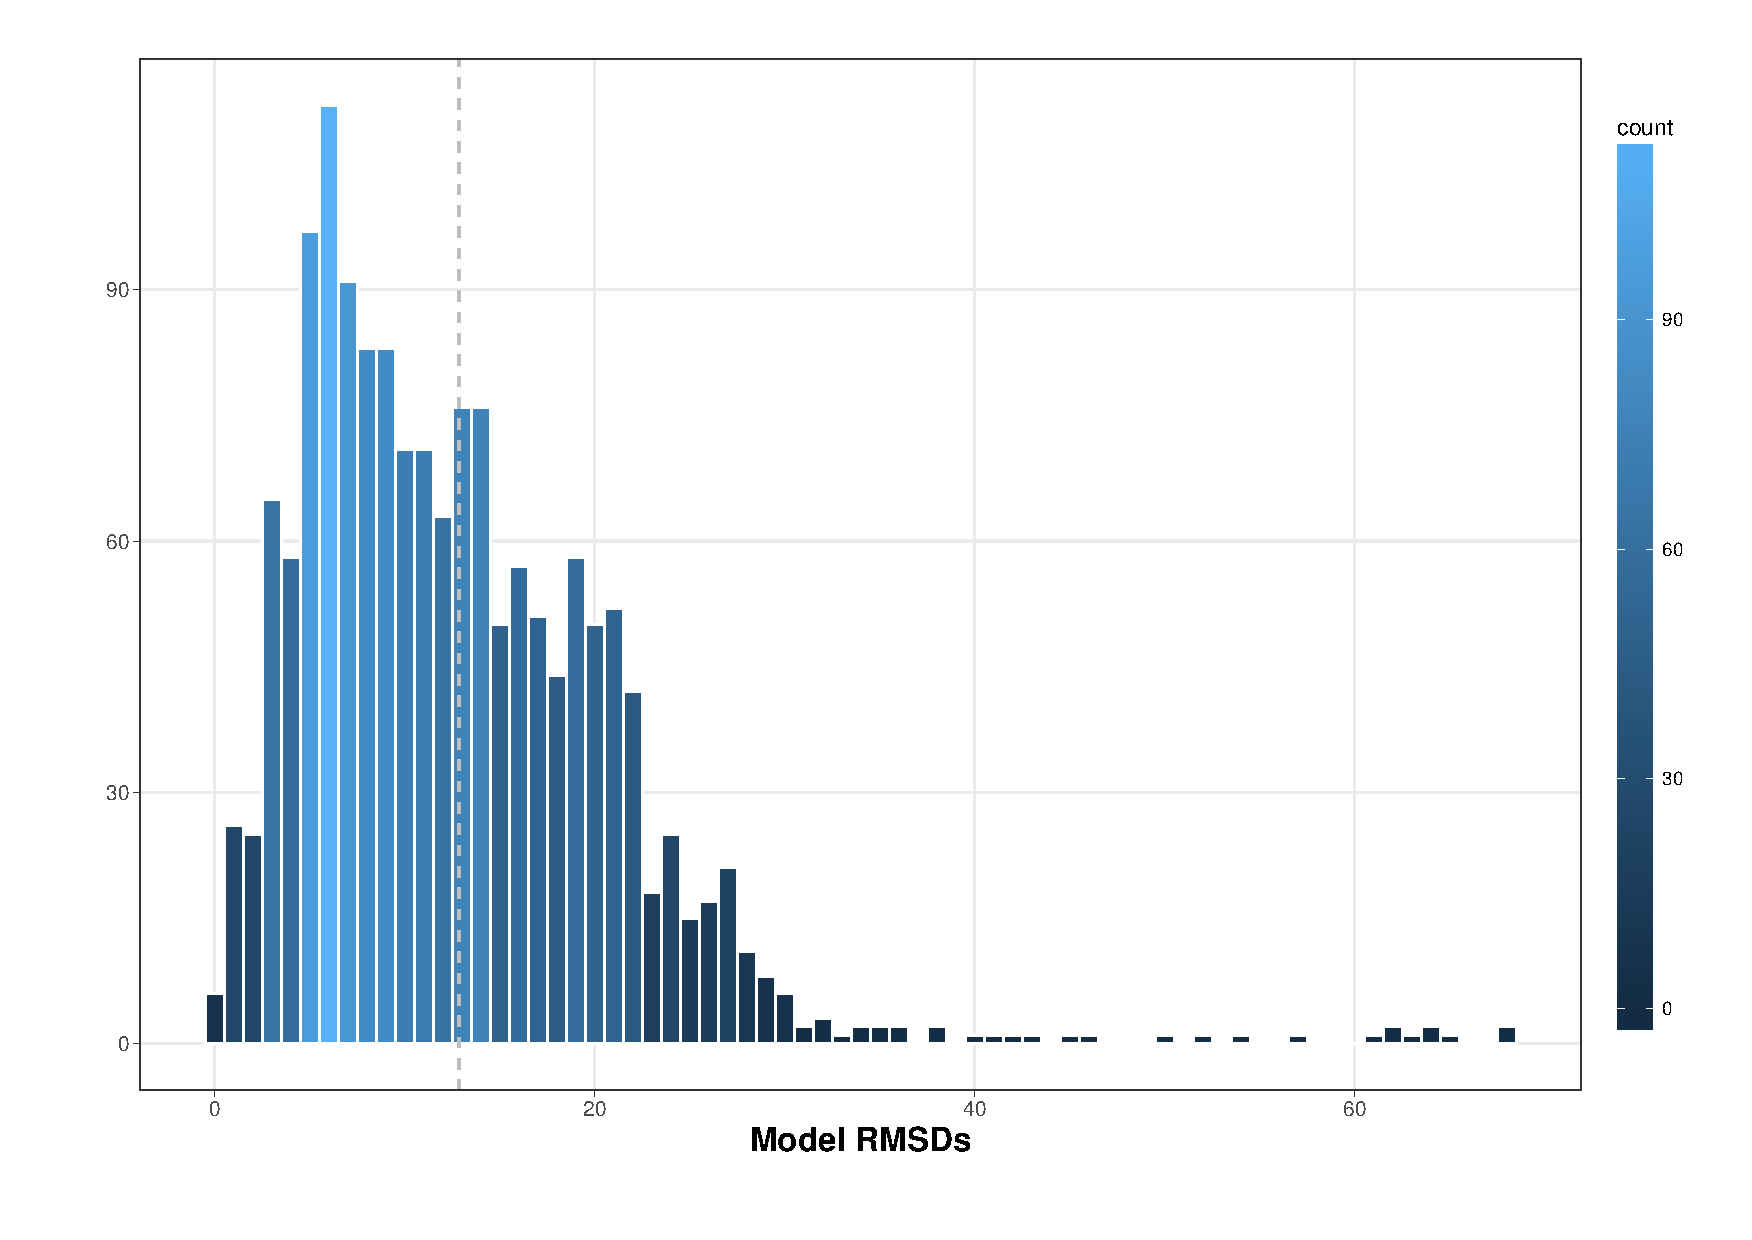
\includegraphics[width=0.9\textwidth]{/Users/joehealey/Documents/Warwick/PhD/Thesis/chapters/chapter3/img/RMSDhist.pdf}
	\captionsetup{singlelinecheck=off, justification=justified, font=footnotesize, aboveskip=10pt}
	\caption[I-Tasser model accuracy distribution - RMSD]{\textsc{\normalsize Distribution of atomic deviations for all simulated models.}\vspace{0.1cm} \newline A histogram of the Root Mean Square Deviation (in \AA{}ngstroms), between a modelled sequence and its closest structural match, as determined by HHSuite. RMSDs were calculated using the MatchMaker function within UCSF Chimera. Reasonable/useful RMSDs of less than $\approx$10 \AA{} are obtained for a significant proportion of the loci simulated. Bars are coloured according to the bin density.}
	\label{rmsdhist}
\end{figure}

That said, despite being the most widely used metric, RMSD is not a perfect measure of structure similarity, as it is prone to large RMSD values (indicative of poor fits) if just a few localised regions are not well matched, even if the protein overall shares similar topology. To this end, I-Tasser also produces calculations of "C-score" (confidence score) and ``TM-score" (template modelling score) \citep{Zhang2005}. I-Tasser provides additional data to assess the best models produced during its molecular dynamics steps, such as the cluster density, which represents the number of times a model passes through a region of 3D modelled space during its molecular dynamics trajectories. Thus the 3D space which is samples most often is likely to represent the conformation of the most favourable models.

\begin{figure}[p]
\centering
\thisfloatpagestyle{IHA-fancy-style}
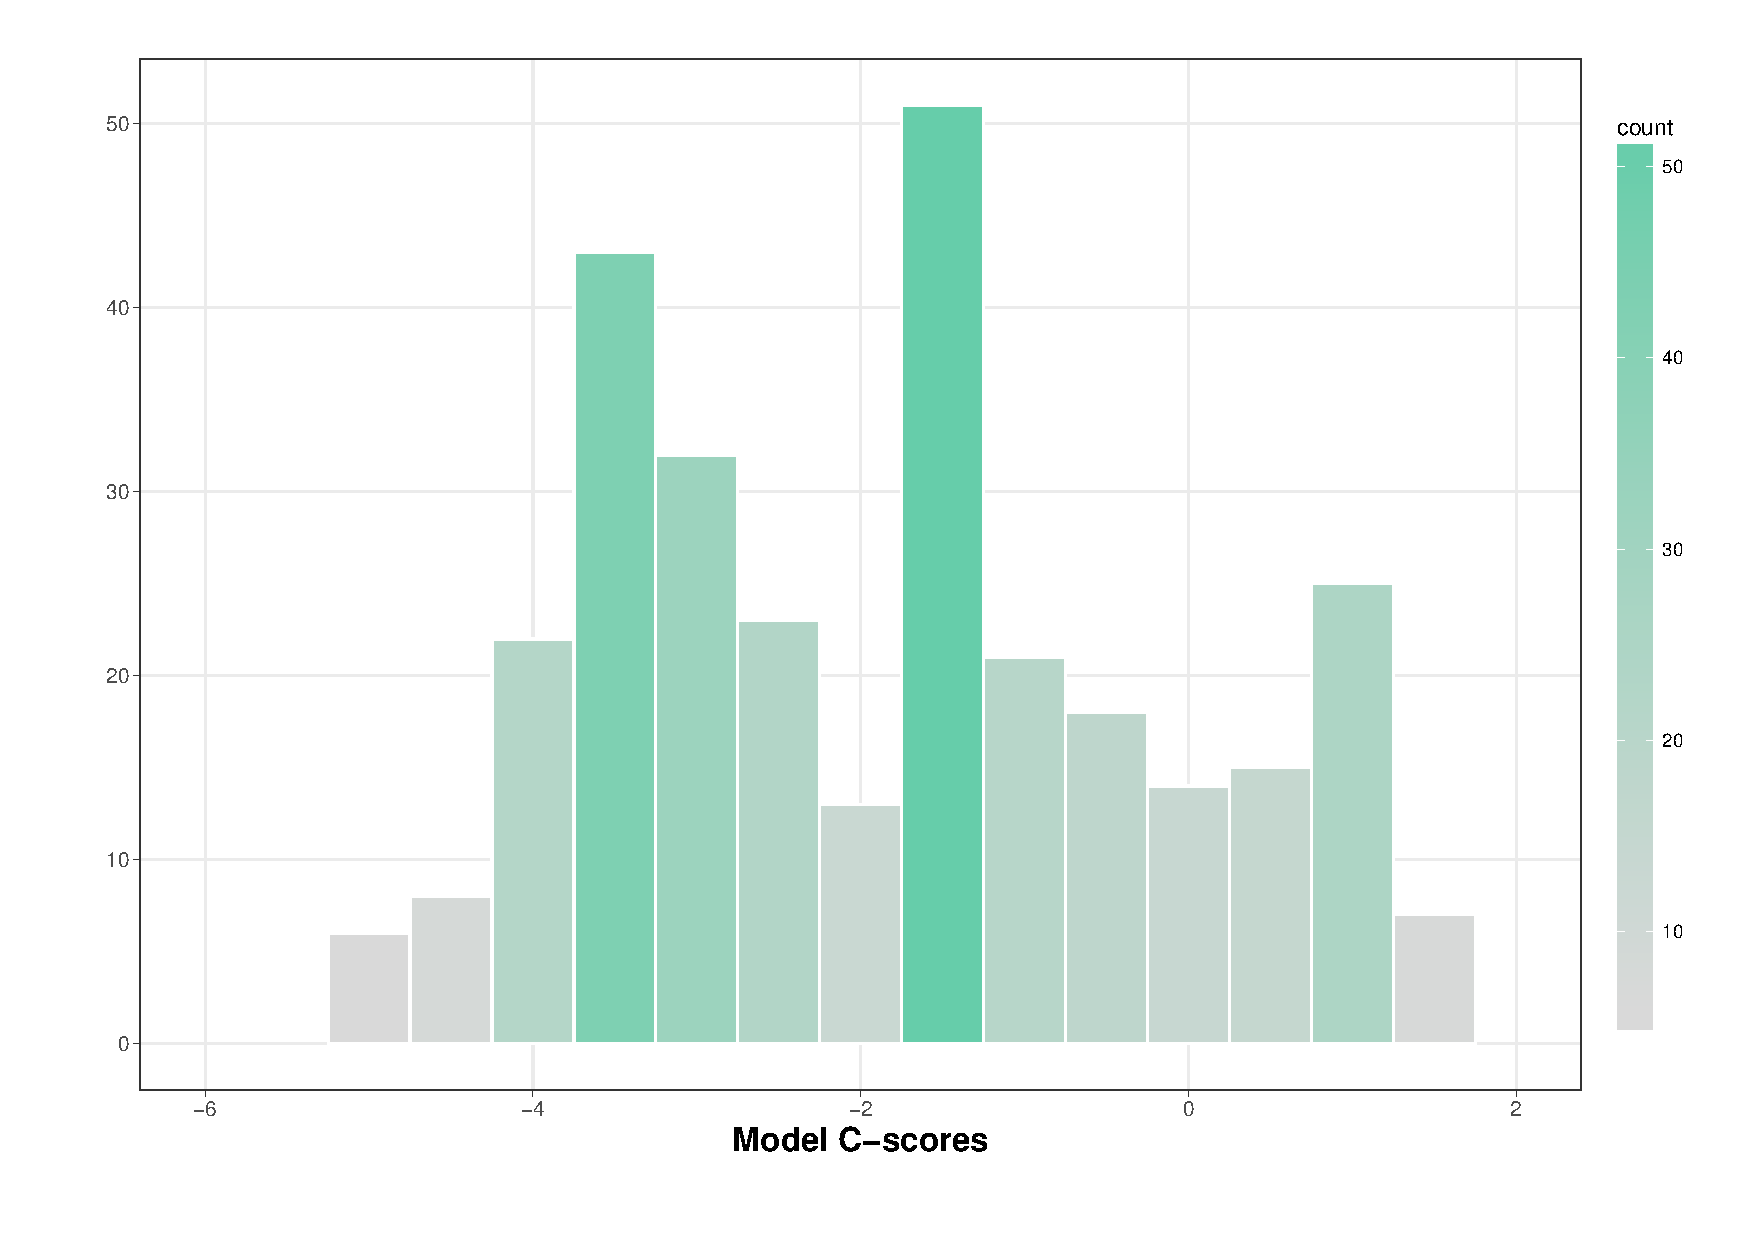
\includegraphics[width=0.9\textwidth, trim={0 30 0 10}, clip]{/Users/joehealey/Documents/Warwick/PhD/Thesis/chapters/chapter3/img/cscores.pdf}
	\captionsetup{singlelinecheck=off, justification=justified, font=footnotesize, aboveskip=7pt}
	\caption[I-Tasser model accuracy distribution - C-score]{\textsc{\normalsize Distribution of the ``C-scores" for all simulated models.}\vspace{0.1cm} \newline A histogram of the ``C-score" from I-Tasser. The C-score is a confidence score calculated internally by I-Tasser based on its confidence in the threading template alignments and convergence of the models. To a rough first estimation, C-scores of greater than approximately -2 indicate reasonable confidence. Approximately half of the models produced therefore have acceptable scores.}
	\label{cscorehist}
\end{figure}
\begin{figure}[p]
\centering
\thisfloatpagestyle{IHA-fancy-style}
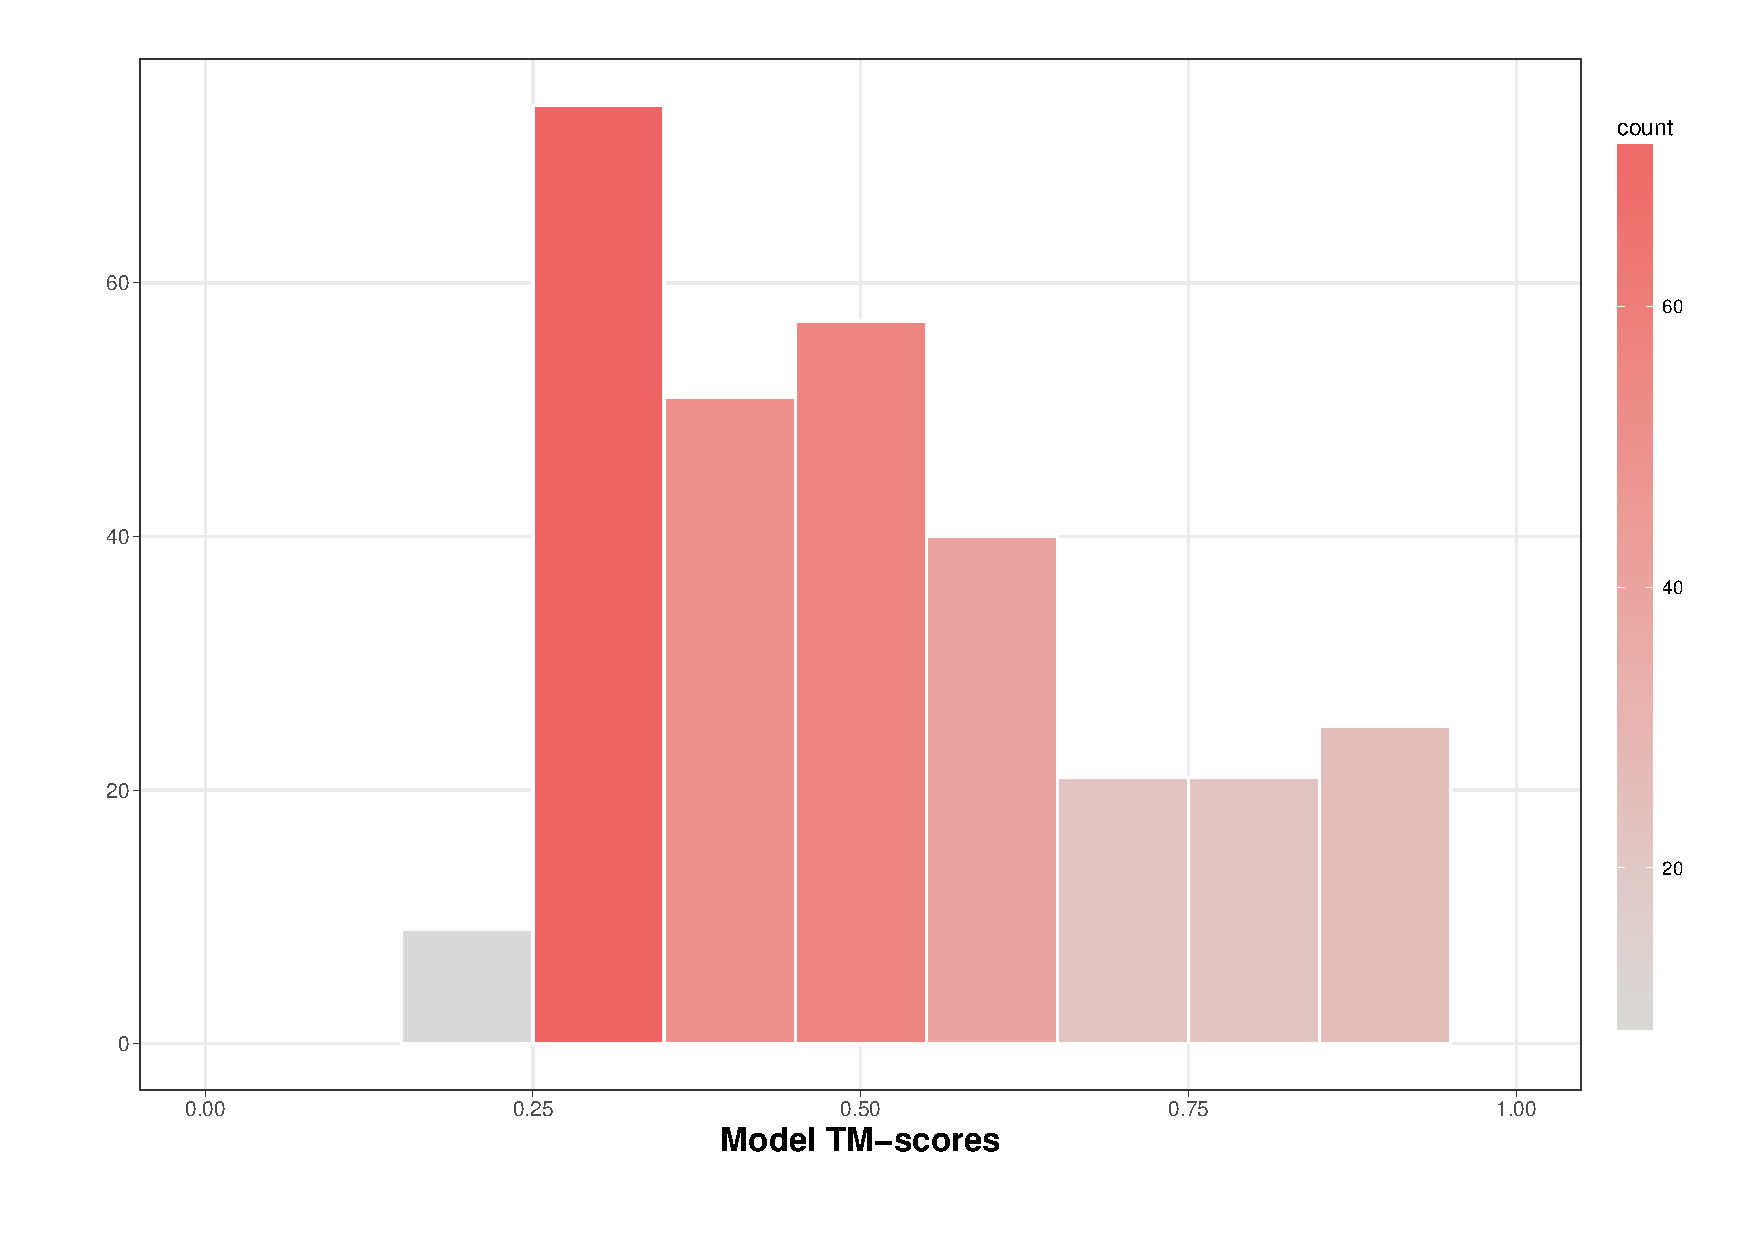
\includegraphics[width=0.9\textwidth, trim={0 30 0 10}, clip]{/Users/joehealey/Documents/Warwick/PhD/Thesis/chapters/chapter3/img/TMscores.pdf}
	\captionsetup{singlelinecheck=off, justification=justified, font=footnotesize, aboveskip=7pt}
	\caption[I-Tasser model accuracy distribution TM-score]{\textsc{\normalsize Distribution of Template Modelling score for all simulated models.}\vspace{0.1cm} \newline A histogram of the TM-score, between a modelled sequence and its closest structural match. TM-scores reflect how well 2 structures match globally, with less susceptibility to local deviations affecting overall score. The vast majority of protein models have TM-scores of greater than 0.25, an acceptable if slightly generous lower bound.}
	\label{tmscorehist}
\end{figure}

There are a large number of models with TM-scores of just over 0.2, (TM-score is in the interval $[0,1]$), which is considered the lower bound on a plausible match between structures \citep{Zhang2005}, suggesting that these protein structures may be of somewhat dubious quality. Roughly half of all modelled proteins have TM scores greater than 0.5 however, and these structures are therefore likely extremely well modelled. This correlates well, as expected, with the C-scores, where higher scores are indicative of better models. C-score is particularly useful when distance based metrics like TM-score and RMSD cannot be used, namely in situations where a template protein could not be identified at all.

It is important to mention however, that despite all these metrics, whether or not a model is useful depends heavily on the question at hand, since models which diverge from the reference structures may still have important/useful information in. Moreover, not all of the metrics correspond perfectly with one another (for instance, some models which have poorer C-scores, actually have good RMSD values. As the epigraph at the start of this chapter suggests, there is no substitute for visually inspecting the models oftentimes, and many of the models are visualised in the remainder of this chapter.

11 of the sequences attempted failed to simulate. Firstly, 8 sequences from the \Pasy{} Kingscliff genome failed to simulate due to the presence of ambiguous amino acids as a result of a lower quality genome assembly. Three proteins were rejected due to being too long - I-Tasser's algorithms have a hard cut-off of 1500 amino acids. 

For the purposes of this chapter, structures are going to be assumed to be predominantly correct (positions of certain loops and small discrepancies notwithstanding). In cases where the simulations are likely spurious they will be noted in the discussion. That is to say, where good templates have been identified and plausible structures have been obtained, the electrostatics, general fold, and any inferences based on these will be assumed to be correct in the absence of truly resolved structures which could reveal unexpected differences.

\clearpage
\subsection{Exploration of the structure of PVCs by functional unit}
%It has been made abundantly clear that it is insufficient to consider sequence similarity alone when comparing structural proteins. Sequences are at liberty to diverge, and if the structure they give rise to is particularly robust, the `space' that the sequence has to drift in is even larger. This is a generally observed phenomenon, but appears to be particularly true for many of the proteins in contractile tail structures. One postulate for this is that phage represent an extremely ancient domain of life, and spend a significant amount of their life cycle outside of the protective environment of the cell they infect. Thus their proteins have evolved over aeons to become particularly stable and robust. The arms race associated with infection cycles has also no doubt driven the diversification of these proteins in an effort to avoid immune mechanisms of their hosts. It has been observed many times in the related literature that, for example, the vgrG/gp5-gp27 spike complex of these caudate systems look almost identical structurally, with many of the same domains identifiable such as the OB-fold, yet may share as little as 12\% protein sequence identity, and due to the slower evolution of proteins sequences attributable codon redundancy, the corresponding DNA sequences may be even less similar.
%
%Consequently, we must make efforts to study the structure as best as possible. In silico methods are improiving all the time, and with more computer power than ever, simulations are becoming routinely feasible. threading approaches are not ideal as they are still too dependent on first identifyin sequence similarity. ab initio approaches allow the structures to be refined without a dependence on the sequence, which should offer an improvement. Structurally conserved proteins with a high degree of robustness should therefore naturally coalesce toward the same structure.

\subsubsection{The PVC tube}
\begin{figure}[h!]
\thisfloatpagestyle{IHA-fancy-style}
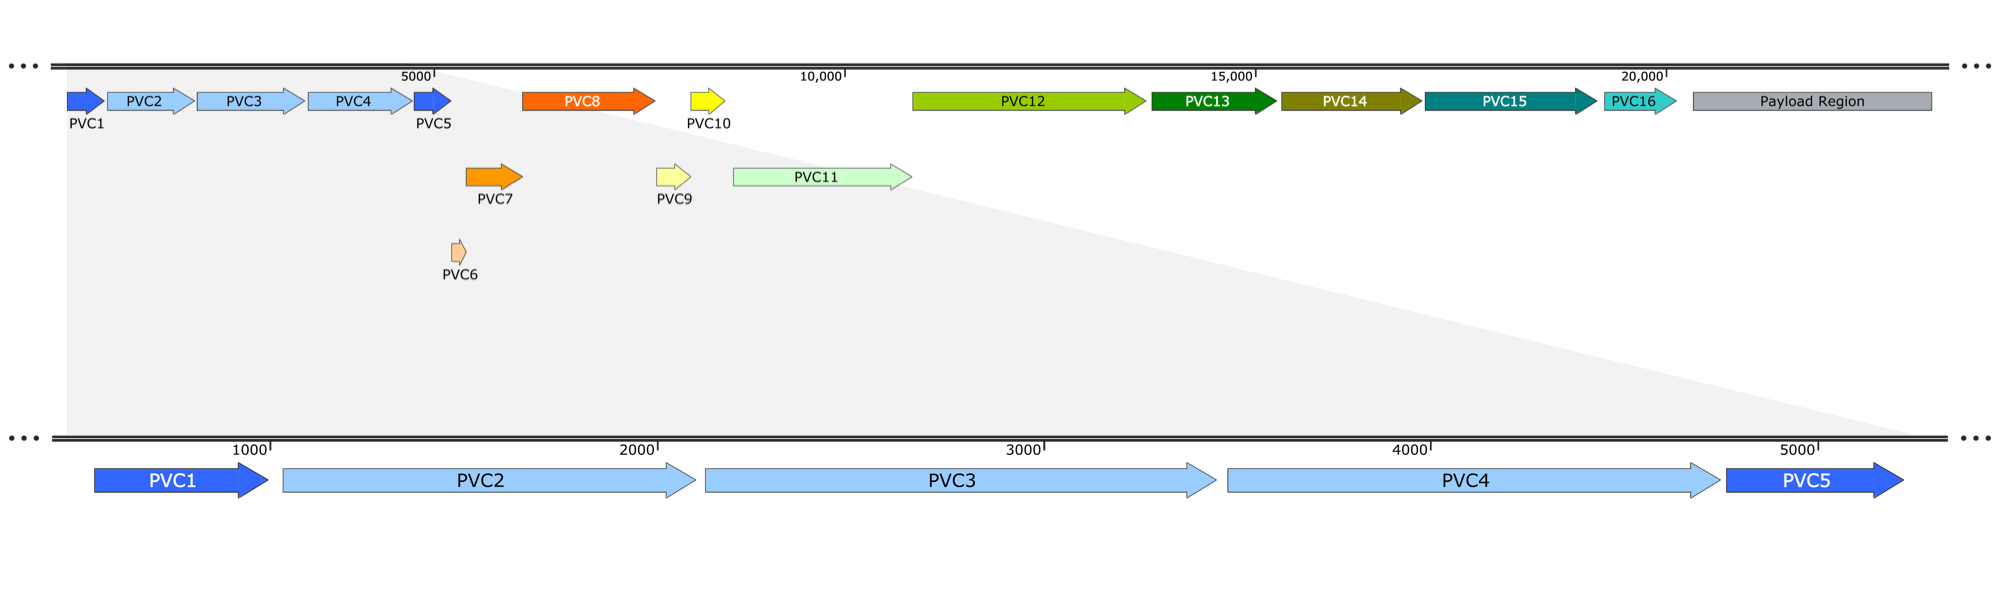
\includegraphics[width=\linewidth]{/Users/joehealey/Documents/Warwick/PhD/Thesis/chapters/chapter3/img/PVC1-5_expanded_map.png}
	\captionsetup{singlelinecheck=off, justification=justified, font=footnotesize, aboveskip=10pt}
	\caption[Tube protein region of a PVC operon]{\textsc{\normalsize The 5 loci that comprise the tube structure of a PVC.}\vspace{0.1cm} \newline The Pnf operon is used as an exemplar of the numbering of loci within an archetypal PVC operon, and 3 colourings are used to demarcate the `functional units' of an operon: blue - tube proteins, orange/yellow - spike complex proteins, green/cyan - the operon `core'. The 5 loci that give rise to the functional unit of the spike complex itself are blown up below as an aid to understanding the operon organisation and the proteins under discussion.}
	\label{PVC1-5map}
\end{figure}


Among the better annotated genes at the outset of this work, the first 5 loci of the PVCs, are predicted to match phage tail tube proteins of various sorts, though the existing annotations were not much more informative than this (for the rest of the operon the vast majority of which were ``hypothetical proteins"). With further inspection, these genes have become consistently annotated as T4-like virus tail tube or baseplate proteins (orthologs of gp6/gp19) and sheath proteins from the recently resolved \emph{Pseudomonas aeruginosa} R-type pyocin. In some previous rounds of annotation, homologies to the Type 6 Secretion Systems of \emph{Edwardsiella tarda}, \emph{Vibrio cholerae}, and \emph{Burkholderia pseudomallei} were also detected for the inner sheath proteins (PVC1 \& 5), which underscores the original notion that PVCs seem to resemble a sort of hybrid, somewhere between a T6SS and a phage in sequence similarity.

From the resolved structure databases and literature, gp19 is known to be the inner sheath of the T4 bacteriophage (as can be seen in PDB IDs 5IV5 and 5W5F \citep{Taylor2016, Zheng2017}), and the outer sheath of PDB ID 3J9Q which corresponds to the resolved pyocin tube structure \citep{Ge2015a}. Over several iterations of homology searches with the HHpred suite, these 3 recent PDB depositions have come to be the most highly similar structures predicted.

\vref{tubehomologs} shows a summarised selection of the orthologues which HHPred has picked up over time. A full list of the most recent orthologies detected can be found in Appendix \vref{structural_appendix}.

\scriptsize
\rowcolors{2}{gray!10}{white}
\begin{tabularx}{\textwidth}{
>{\centering\arraybackslash} m{0.11\textwidth}
>{\centering\arraybackslash} m{0.11\textwidth}
>{\raggedright\arraybackslash} X
>{\raggedright\arraybackslash} X
}
\hiderowcolors
\captionsetup{singlelinecheck=off, justification=justified, font=footnotesize, belowskip=5pt}
\caption[HHPred hit summary for PVC1-5]{\textsc{\normalsize HHPred orthology summary for the tail tube proteins.}\vspace{0.1cm} \newline A summary of homology matches via HHPred for the first 5 PVC loci. The hits have varying degrees of confidence but have Probabilities greater than 60\% and E-Values of less than \sn{1}{-5}. They represent a `collapsed' set of common hits from all the variants for each locus. Hit scores for the inner sheath proteins (PVC1 and 5) are consistently lower than for the outer sheath proteins (PVC2-4) - all scores for the most recent analysis can be found in Appendix \vref{structural_appendix}.}\\
\label{tubehomologs}\\
Locus & PDB ID Hit & Structure & Component \\
\hline\hline
\showrowcolors
\hline

\rowcolor{white!10}                              & 5IV5 & Bacteriophage T4 & Baseplate wedge protein (gp6) \\ 
\rowcolor{white!10}                              & 5W5F & Bacteriophage T4 & Tail tube protein (gp19) \\
\rowcolor{white!10}                              & 3EAA & T6SS             & Inner sheath protein (Hcp/TssD)\\
\rowcolor{white!10} \multirow{-4}{*}{PVC1 \& 5*} & 4TV4 & T6SS             & Inner sheath protein (Hcp/TssD)\\
\rowcolor{gray!10}  PVC2, 3, \& 4                & 3J9Q & R-type Pyocin    & Outer sheath protein \\

\end{tabularx}
\hrule
\vspace{0.1cm}
{\tiny \noindent * PVC5 attracts the same 3 homology matches as PVC1, plus 4TV4.}
\normalsize

Figures \vref{PVC1comparisons} and \vref{PVC2comparisons} showcase the similarities and differences in structure between the first 5 PVC loci and their nearest structural homologs either as determined via HHPred or previously shown in the literature. In addition, they also show a simulated structure for the Antifeeding Prophage equivalent locus. The Afp is the closest orthologue when only DNA or amino acid sequence is considered, but no resolved structure exists (and therefore cannot be picked up by HHPred when using HMMs of the PDB database). \vref{PVC2comparisons} replicates this for an example of the outer sheath proteins.

Rather than show all the PVC loci compared to their homologs, where the PVC loci are similar, one example is shown (as in \vref{PVC1comparisons}) and then all the PVC variants are compared with one another in the subsequent \vref{PVC1-5_conservation}.

The inner sheath proteins from all these structures form a conserved pair of anti-parallel $\beta$-sheets which are sandwiched together approximately perpendicular to one another (with the exception of the T4 baseplate protein which appears to be an erroneous homology). They all exhibit a lower right hand extension positioned almost exactly in the centre of the amino acid chain (cyan/aquamarine) which would overlap the monomer adjacent to it within the tube hexamer. In the case of the T4 gp19 tube protein (chain F from PDB ID 5IV5), this is quite extended, along with a much longer protruding C-terminus (dark blue).

The matched PDB ID 5IV5 is the entire baseplate complex of T4, including part of the tube (and encapsulates PDB ID 5W5F, so there is a slightly redundant match), from the T4 phage. It seems unusual that many of the proteins match (at the sequence and secondary structure level) to chains within the model which are \emph{not} the tube, instead forming part of the baseplate complex, primarily gp6. It is clear from looking at the structures visually that these proteins are definitively homologues of the inner sheath proteins. On further inspection of the specific sequence matches detected by HHPred, it appears that what may have transpired is an error in the annotation of gp6 being attributed to some of the gp19 chains within the enormous 5IV5 PDB complex.

Inset in each figure is a pairwise distance matrix for alignments of the tube orthologues. Interestingly, though perhaps unsurprisingly, the sequence identity between the PVC and Afp is significantly better (a lower distance) than it is between either of them and the T6SS, T4 or Pyocin, despite the structures being extremely good matches, further reinforcing the message of this chapter that the sequence alone is insufficient to fully capture the subtleties of the evolution of these structures. Excluding the erroneous gp6 orthology, the remaining structures can be superimposed to an accuracy of 1.2 \AA{} or less.

For the outer sheath proteins, of which there are curiously 3 in most operons, but PVC3 can be deleted, there is no ambiguity in their sequence matches, all having orthology to the R-type pyocin outer sheath under the PDB ID 3J9Q. The structures of the PVC2 locus from the ``Pnf" operon, and equivalent outer sheath proteins from other structures are also shown as in \vref{PVC1comparisons}, though they are less compelling matches than the pyocin at the sequence/HMM level (with the exception of the Afp, which is not detected by HHPred as the structures are unresolved).

The outer sheath proteins are characterised by 2 outstretched termini which interlace with the adjacent monomers to form the contractile mesh over the rigid inner tube. In the case of the T4 tube, it's C-terminus actually forms an additional domain known as the ``protease resistant fragment", which the other structures lack \citep{Aksyuk2009}. The Type 6 Secretion System is unique amongst T4-like caudate structures, having a second outer sheath protein (TssB and TssC - known as VipA and VipB in the case of \emph{V. cholerae}), making the equivalent outer tube a heterododecamer. All the structures contain a pair of helices extending vertically which neighbour a pair of anti-parallel strands/sheets, that form the attachment interface to the inner tube electrostatically \cite{Ge2015a}.

Curiously, the 20 \AA{} Afp EM map depicted in \vref{afpstructure} seems to show protrusions of the sheath monomers radially, though the sheath proteins very closely match that of the R-type pyocin, as do the PVCs, and the R-type pyocin map lacks any such protrusions. Similarly, preliminary cryoEM data for the PVCs suggests a lack of any protrusions too. This might be indicative of an unknown third protein augmenting the exterior of the sheath, somewhat like the T6SS dodecameric arrangement.

The outer sheaths of all the non-T4, released/secreted, caudate structures are therefore much simpler proteins, representing perhaps a minimal functional unit capable of exerting the contraction, which is then decorated with domains such as the protease resistant fragment of T4 to confer further features to the sheath.

The pairwise sequence distances between the outer sheaths tell a similar story to the inner sheaths, with the PVC and Afp being the closest by some margin, compared to the remaining structures. However, the sequence distance is greater between the PVCs/Afps outer sheaths than it was for the inner sheaths. This will be due in part to the fact that the proteins are longer, but it seems that the surfaces of caudate apparatuses are open to modification, possibly to cope with different environmental stresses, or at the very least have some sequence redundancy. All proteins can be superimposed to an accuracy of less than 1.2 \AA, despite significant sequence differences.

\begin{figure}[p]
 \thisfloatpagestyle{augment}
\begin{subfigure}[H]{\textwidth}
  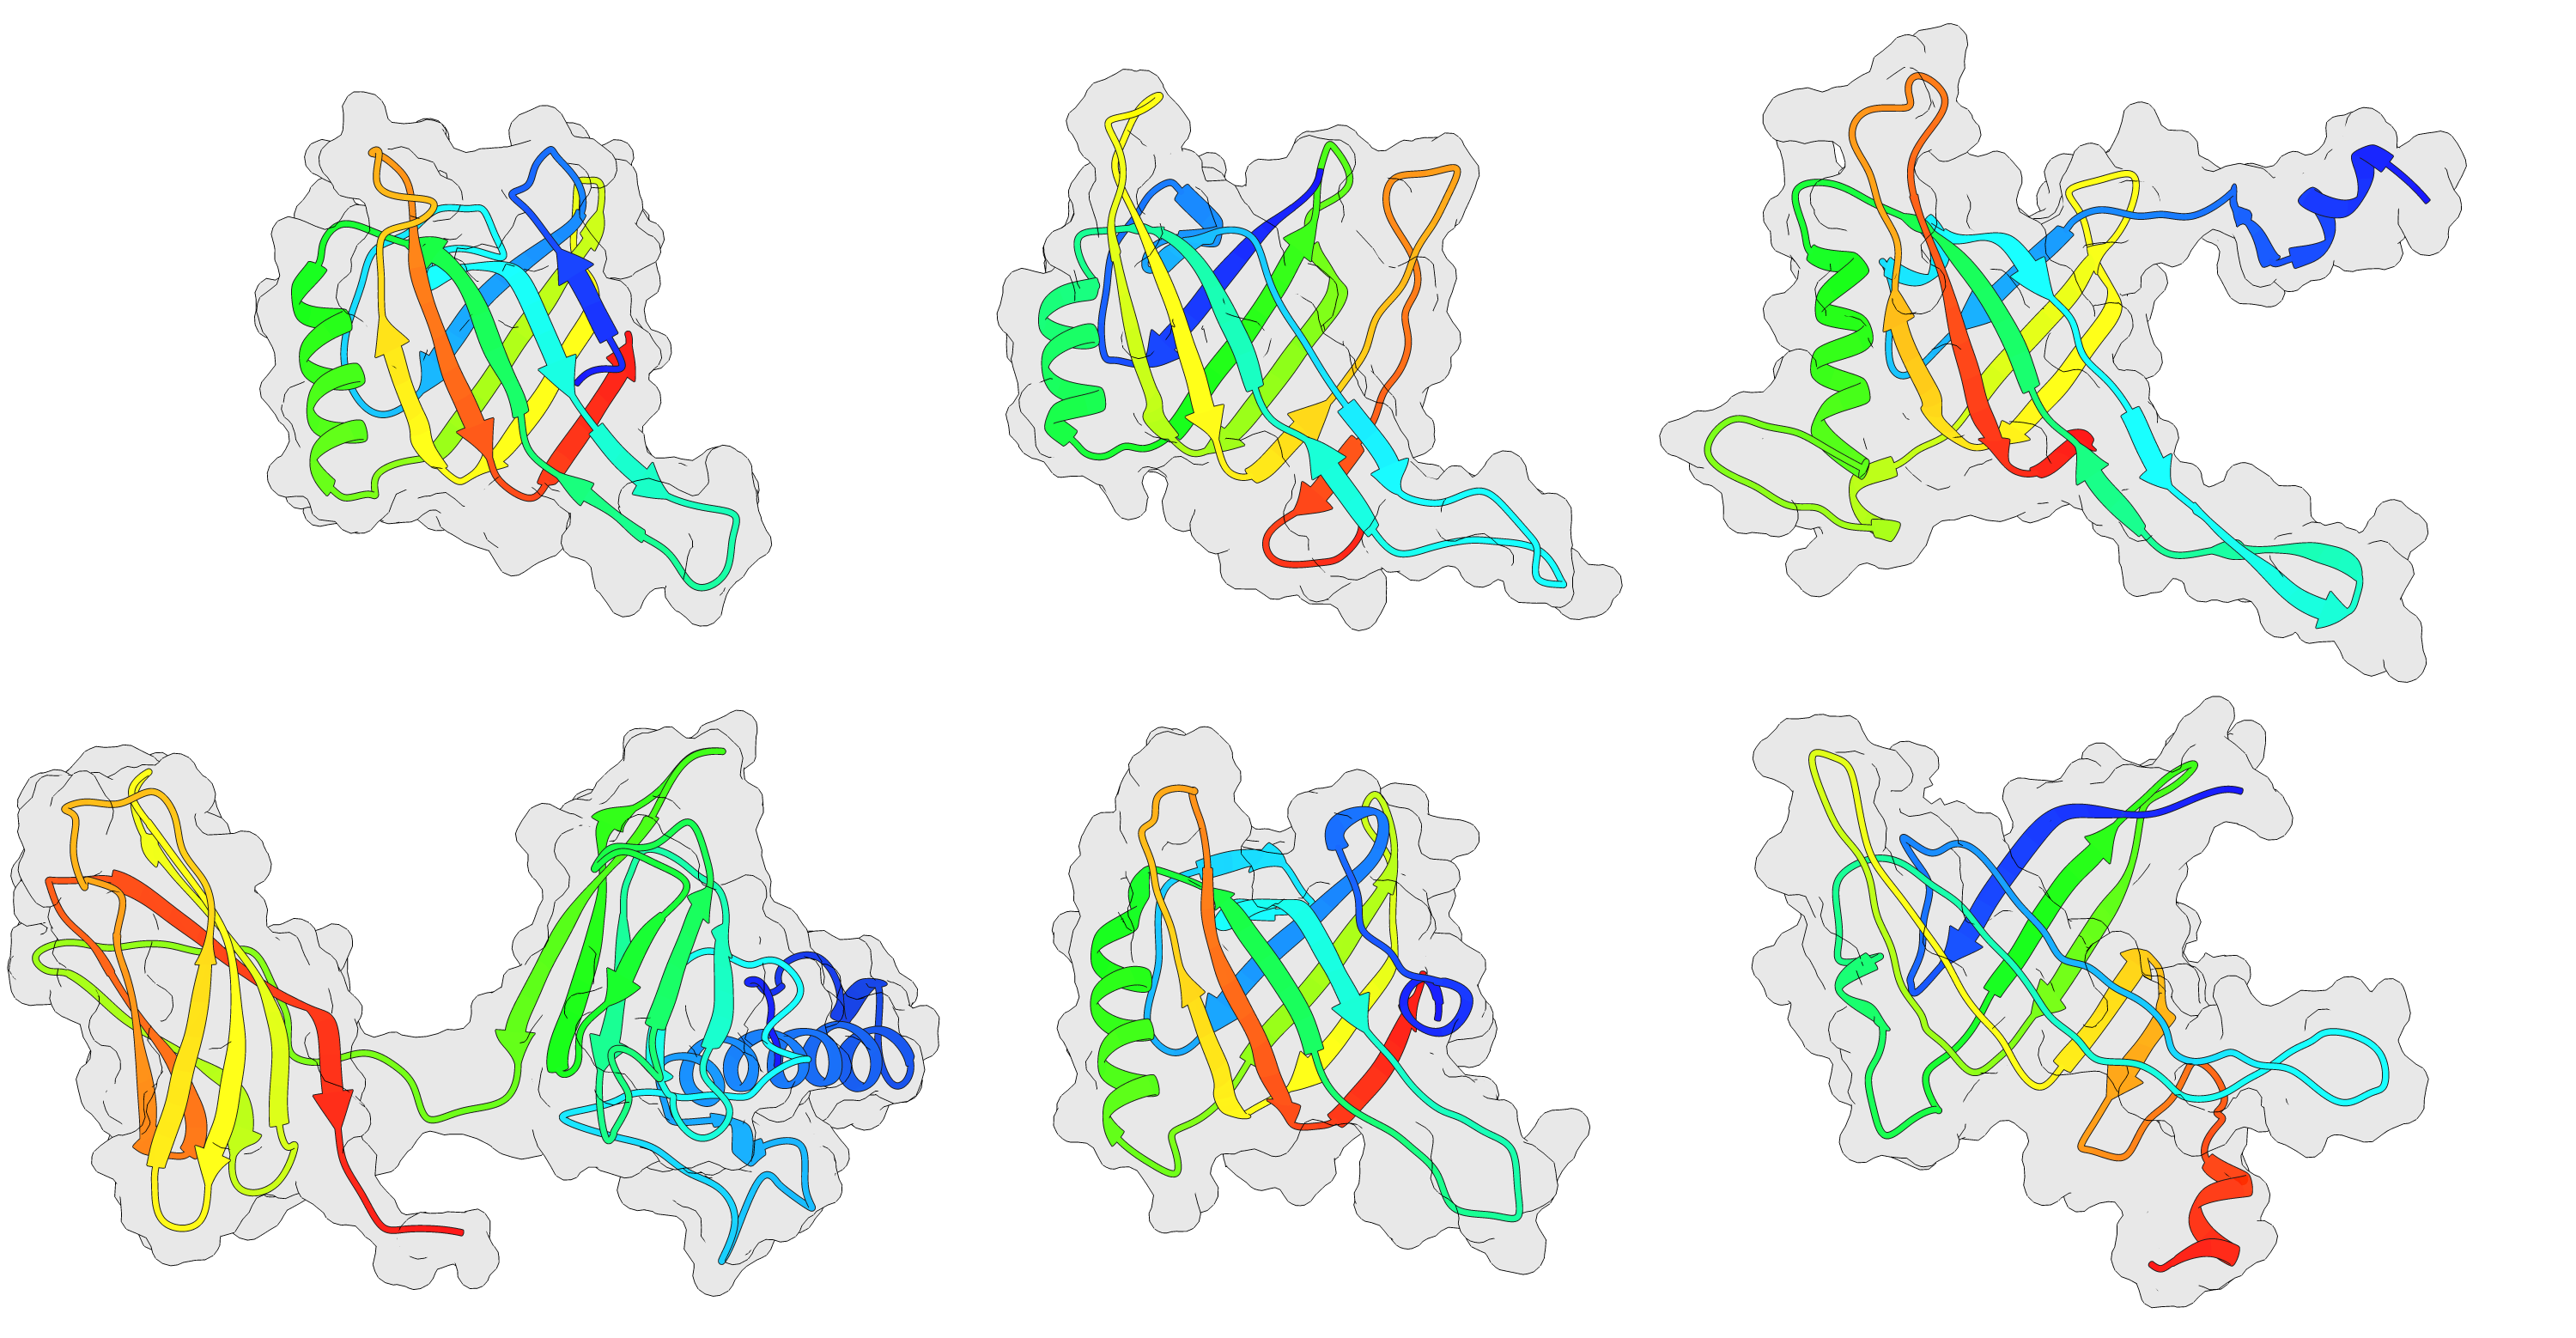
\includegraphics[width=\textwidth, trim={30 0 30 0}, clip]{/Users/joehealey/Documents/Warwick/PhD/Thesis/chapters/chapter3/img/PVC1_homolog_comparison.png}
 \put(-370,115){\small \centering PVC Simulation}
 \put(-227,115){\small \centering T6SS}
 \put(-105,115){\small \centering T4 Tube}
 \put(-370,-5){\small \centering T4 Baseplate}
 \put(-241,-5){\small \centering Afp Simulation}
 \put(-100,-5){\small \centering Pyocin}
\end{subfigure}
\begin{subfigure}[H]{\textwidth}
\tiny
\rowcolors{2}{gray!10}{white}
\begin{tabularx}{1.01\textwidth}{CCCCCCC}
\rowcolor{white!10}\multicolumn{7}{c}{Distance Matrix} \\
\hline
Model  & \multicolumn{6}{c}{Pairwise Distances}\\
\hline\hline
PVC                   & 0.000000 & 0.872483 & 0.885906 & 0.865772 & 0.255034 & 0.892617 \\
T6SS                  & 0.872483 & 0.000000 & 0.895706 & 0.876471 & 0.865772 & 0.892857 \\
T4 Tube               & 0.885906 & 0.895706 & 0.000000 & 0.846626 & 0.879195 & 0.877301 \\
T4 Baseplate          & 0.865772 & 0.876471 & 0.846626 & 0.000000 & 0.852349 & 0.880952 \\
Afp                   & 0.255034 & 0.865772 & 0.879195 & 0.852349 & 0.000000 & 0.899329 \\
Pyocin                & 0.892617 & 0.892857 & 0.877301 & 0.880952 & 0.899329 & 0.000000 \\
\end{tabularx}
\end{subfigure}  
 \captionsetup{singlelinecheck=off, justification=justified, font=footnotesize, aboveskip=20pt}
 \caption[PVC1 homolog comparisons]{\textsc{\normalsize Comparisons of the structure of PVC locus 1 to orthologous proteins.}\vspace{0.1cm} \newline An example model of PVC locus 1 from the PVCPnf operon of \Pasy{} ATCC43949. Here the structure is compared to (from top left to bottom right) the Hcp protein (5OJQ chain W) of the \emph{V. cholerae} T6SS, gp19 (5W5F chain V) from the T4 bacteriophage, gp6 also from T4 (5IV5 chain F), a simulated Afp1 structure from \emph{S. entomophila}, and an interior sheath monomer from the R-type pyocin (3J9Q chain V) from \emph{P. aeruginosa}. Models are shown `rainbow' coloured, from one terminus to the other, with a molecular surface `ghost'. It is evident that the 2 T4 proteins, despite being frequent sequence based matches to PVC1 (and 5), are not the closest matches in terms of structural conformation. The 3D model to accompany this page shows superimposed $\alpha$-carbon chain traces for all the structures (though without the T4 baseplate as its superposition is poor) - the PVC protein is rendered in thicker red wires/pipes, and the homologs in various monochrome shades. The inset table shows the all-vs-all pairwise alignment distances for the amino acid chains depicted }
	\label{PVC1comparisons}
\end{figure}

\begin{figure}[p]
 \thisfloatpagestyle{augment}
 \begin{subfigure}[H]{\textwidth}
 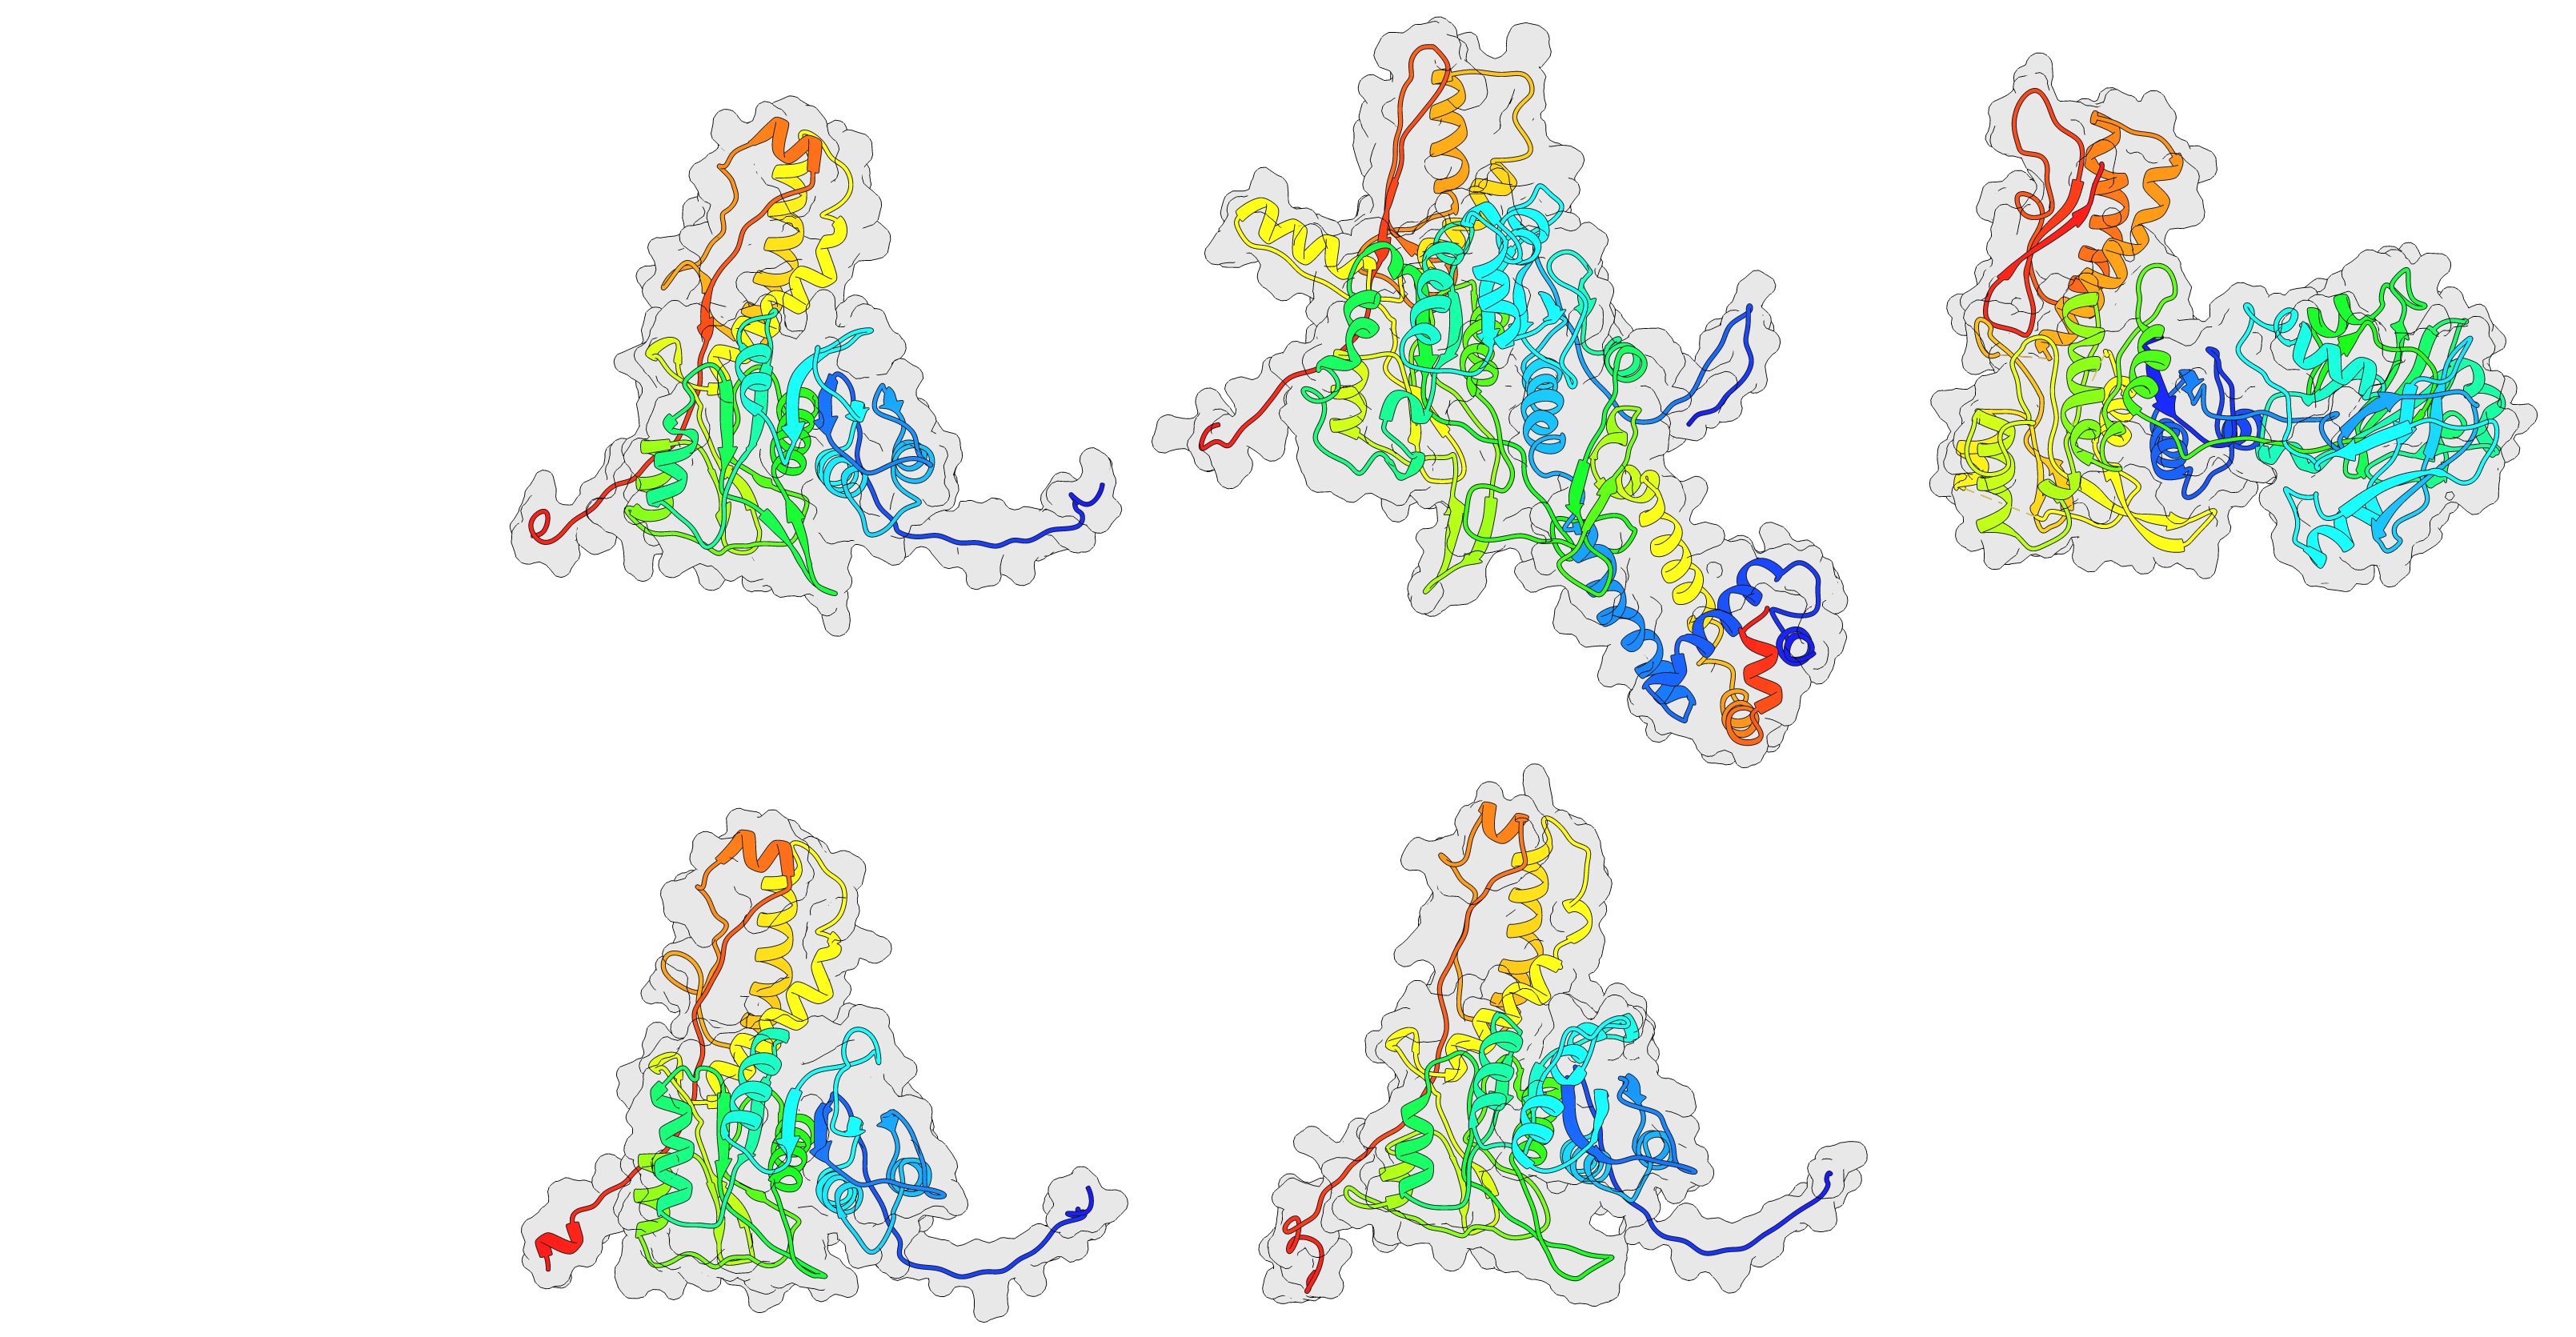
\includegraphics[width=\textwidth, trim={150 0 0 0}, clip]{/Users/joehealey/Documents/Warwick/PhD/Thesis/chapters/chapter3/img/PVC2_homolog_comparison.png}
 \put(-400,125){\small PVC Simulation}
 \put(-295,145){\small T6SS (A) \customarrow{2pt}{200}}
 \put(-250,125){\small T6SS (B) \customarrow{2pt}{200}}
 \put(-105,125){\small T4 Tube}
 \put(-400,-10){\small Afp Simulation}
 \put(-230,-10){\small Pyocin}
 \end{subfigure}
\begin{subfigure}[H]{\textwidth}
\tiny
\rowcolors{2}{gray!10}{white}
\begin{tabularx}{1.01\textwidth}{CCCCCCC}
\rowcolor{white!10}\multicolumn{7}{c}{Distance Matrix} \\
\hline
Model  & \multicolumn{6}{c}{Pairwise Distances}\\
\hline\hline
PVC       & 0.000000 & 0.890141 & 0.851613 & 0.856338 & 0.539548 & 0.845070 \\
T6SS VipA & 0.890141 & 0.000000 & 0.864516 & 0.883721 & 0.892655 & 0.898701 \\
T6SS VipB & 0.851613 & 0.864516 & 0.000000 & 0.845161 & 0.851613 & 0.864516 \\
T4        & 0.856338 & 0.883721 & 0.845161 & 0.000000 & 0.870056 & 0.875325 \\
Afp       & 0.539548 & 0.892655 & 0.851613 & 0.870056 & 0.000000 & 0.838983 \\
Pyocin    & 0.845070 & 0.898701 & 0.864516 & 0.875325 & 0.838983 & 0.000000 \\


\end{tabularx}
\end{subfigure}  
 \captionsetup{singlelinecheck=off, justification=justified, font=footnotesize, aboveskip=20pt}
 \caption[PVC2 homolog comparisons]{\textsc{\normalsize Comparisons of the structure of PVC locus 2 to orthologous proteins.}\vspace{0.1cm} \newline An example model of PVC locus 2 from the PVCPnf operon of \Pasy{} ATCC43949. Here the structure is compared to (from top left to bottom right) the VipA/VipB proteins (5OJQ chains c and m) of the \emph{V. cholerae} T6SS, gp18 (3J2N chain U) from the T4 bacteriophage, a simulated Afp2 structure from \emph{S. entomophila}, and an outer sheath monomer from the R-type pyocin (3J9Q chain A) from \emph{P. aeruginosa}. The T6SS structure uniquely comprises 2 distinct chains, along with some sequence extensions to the main chain. The T4 gp18 contains a considerable augmentation to its C-terminus consistent with protrusions that can be seen in \vref{t4structure}. Models are shown `rainbow' coloured, from one terminus to the other, with a molecular surface `ghost'. The 3D model to accompany this page shows superimposed $\alpha$-carbon chain traces for all the structures - the PVC protein is rendered in thicker red wires/pipes, and the homologues in various monochrome shades. The inset table shows the all-vs-all pairwise alignment distances for the amino acid chains depicted.}
	\label{PVC2comparisons}
\end{figure}


\myparagraph{Structural comparisons of duplicated and triplicated tube proteins}\label{duptrip}
An unanswered question is why \emph{Photorhabdus} has managed to maintain so many copies of what appear to be highly paralogous proteins in the tube region. Not only are the proteins paralogous within a single operon, but multiplied up by 5 or 6 times to account for the other operons, and somehow proteins with as many as 10 or more copies are somehow well preserved, when it might be expected that they would be open to drift.

\vref{PVC1-5_conservation} demonstrates the structural and sequence similarities between all 5 inner and outer sheath loci from the Pnf operon in \Pasy{} ATCC43949. There are some subtle structural differences (spans of loop structure etc.) between the loci, though they generally agree very well and this may be a result of the stochasticity in the molecular dynamics trajectories calculated by I-Tasser. PVC locus 1 does exhibit greater sequence variability compared to its `compatriot' PVC locus 5, though its overall fold is the same.

To explore this further, a comparison is made in \vref{PVC1-5_leastsimilar} between the least similar paralogues, as determined by their distances in the guide tree that accompanies the alignments, to show the most extreme differences (alignments can be found in Chapter \vref{bioinformatics_appendix}). In both cases (PVC1 and PVC5) the ``Lumt" operon from \Pasy{} Kingscliff and ATCC43949 respectively, present one of the pair of least similar sheath proteins. For the counterpart PVC1, the least similar paralogue is the inner sheath from the ``Cif" operon of \Pasy{} ATCC43949, and for PVC5 it is the tube protein of the ``Pnf" operon from the same genome.

\begin{landscape}
\begin{figure}[p]
 \thisfloatpagestyle{IHA-fancy-style}
 \centering
 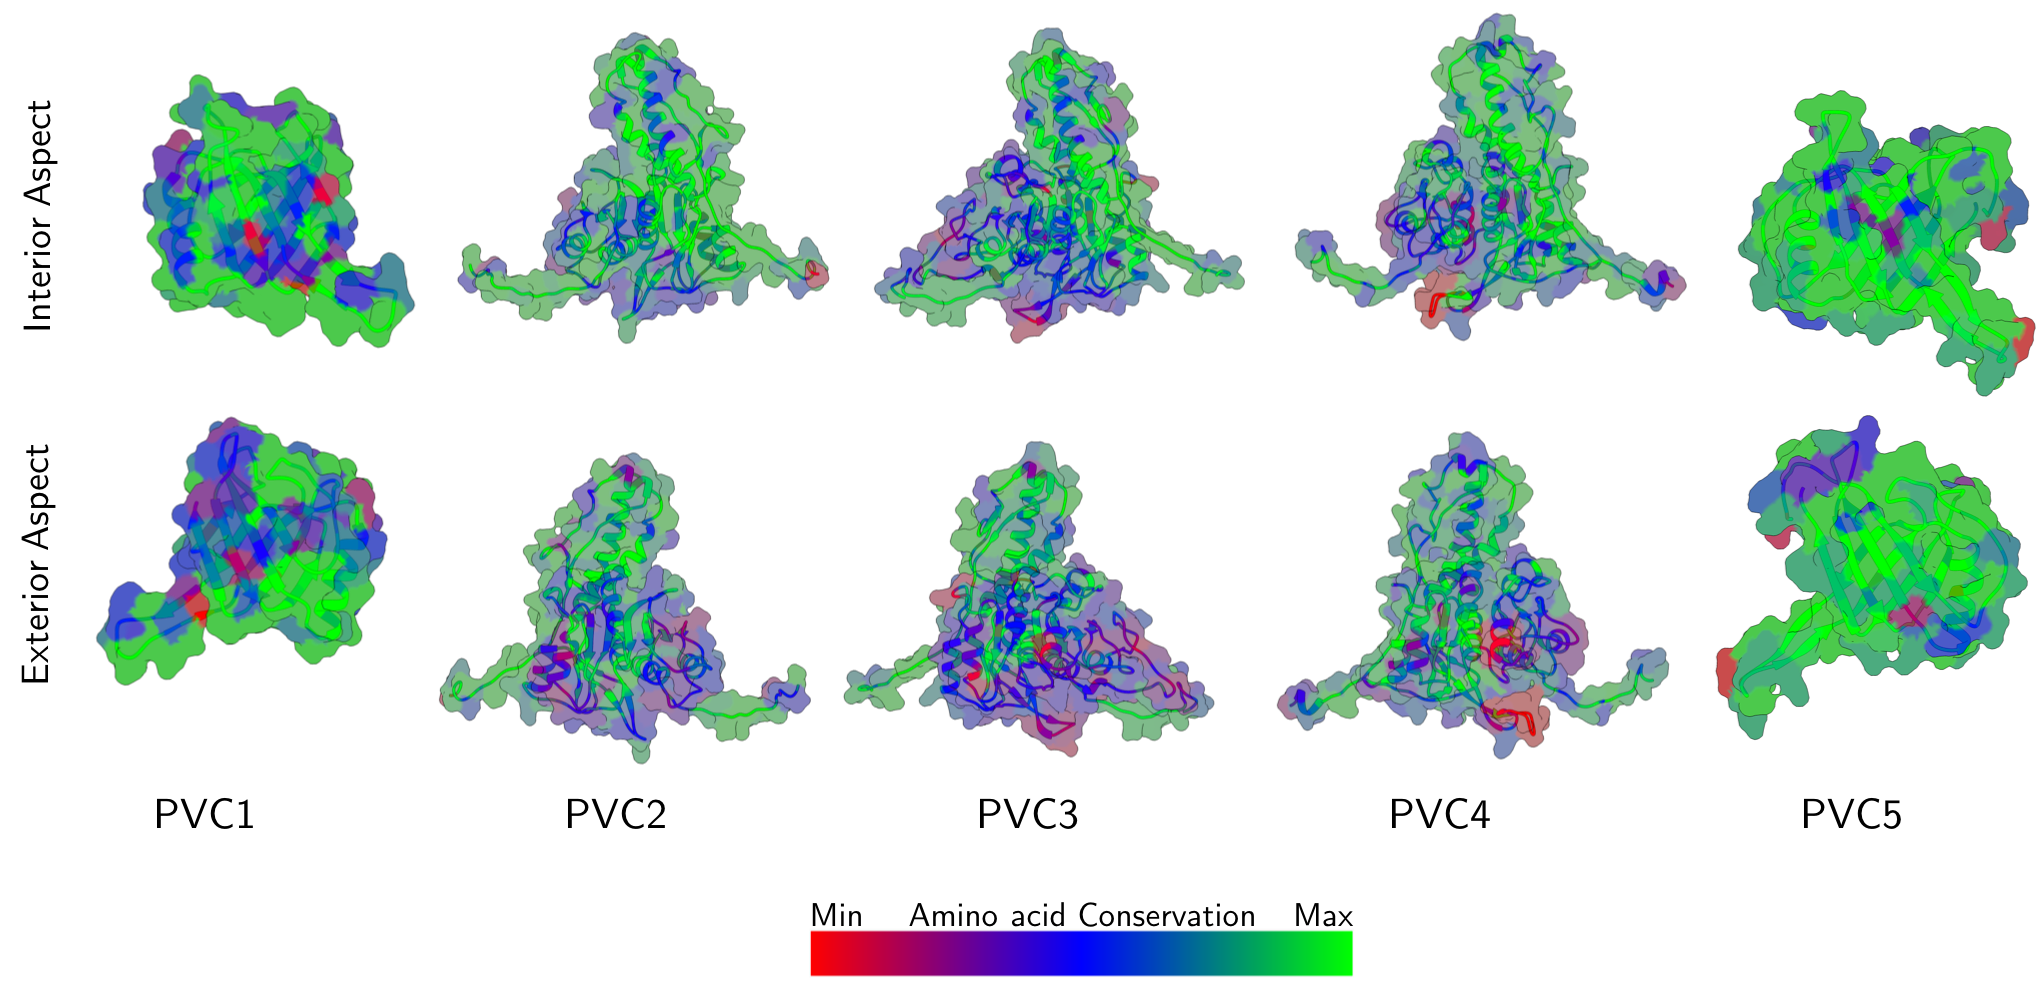
\includegraphics[width=\linewidth, trim={0 0 0 0}, clip]{/Users/joehealey/Documents/Warwick/PhD/Thesis/chapters/chapter3/img/PVC1-5_composite.png}
 \captionsetup{singlelinecheck=off, justification=justified, font=footnotesize, aboveskip=10pt}
 \caption[PVC1 to PVC5 paralogue conservation comparison]{\textsc{\normalsize Comparisons of sequence conservation in inner and outer sheath paralogues.}\vspace{0.1cm} \newline Models of PVC1 to PVC5 for the Pnf operon are shown as front and rear rotations, coloured according to their per-column sequence conservation (as per the sequence alignments in Appendix \ref{bioinformatics_appendix}); rendered from high (green), to low (red), as per the inset scalebar. Structural differences are minimal, and sequence conservation is generally high, though PVC1 is slightly more variable (more blue sites) than its paralogue PVC5. Of the outer sheath proteins, the interior aspect is better conserved than the exterior, and all 3 loci exhibit increased sequence diversity.}
	\label{PVC1-5_conservation}
\end{figure}

\begin{figure}[p]
 \thisfloatpagestyle{IHA-fancy-style}
 \centering
  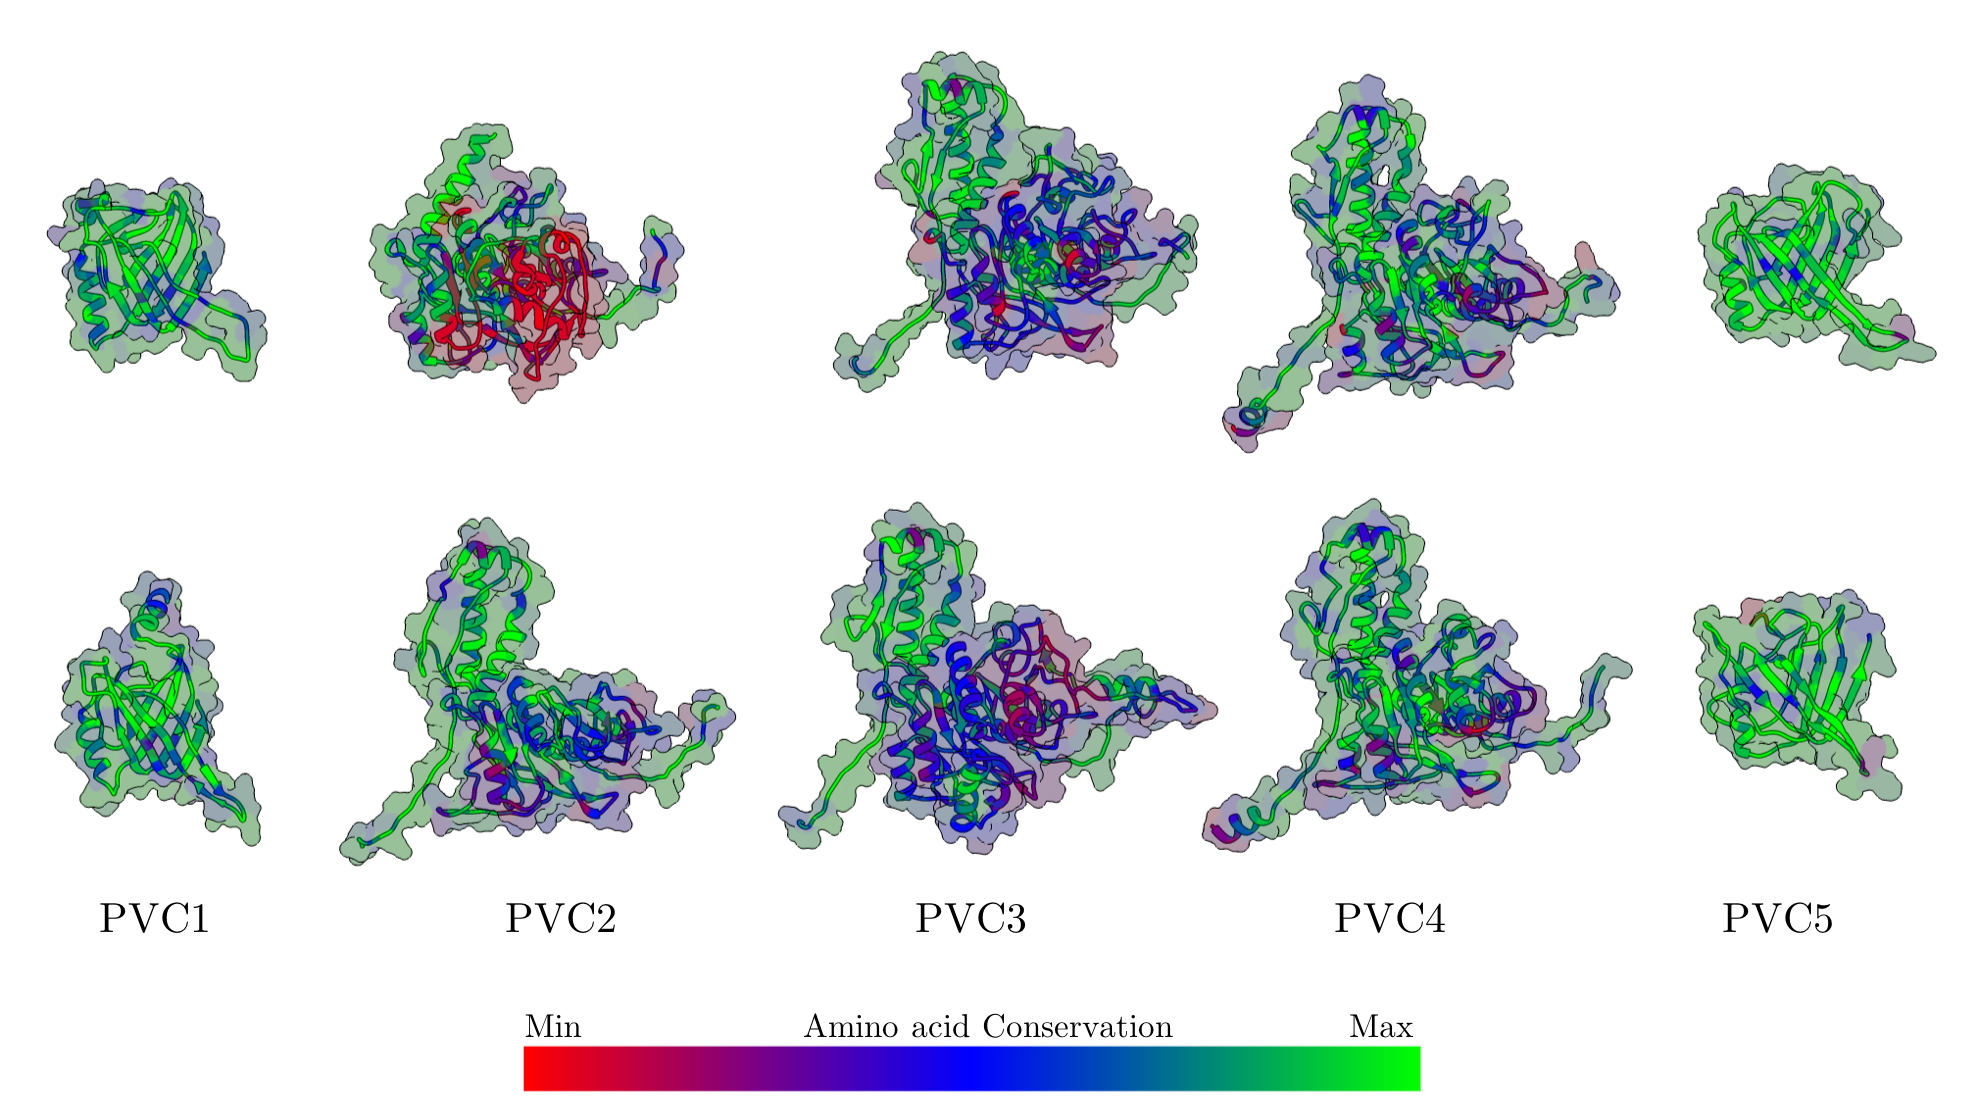
\includegraphics[width=\linewidth, trim={10 10 20 30}, clip]{/Users/joehealey/Documents/Warwick/PhD/Thesis/chapters/chapter3/img/PVC1-5_leastsimilar_composite.png}
 \captionsetup{singlelinecheck=off, justification=justified, font=footnotesize, aboveskip=10pt}
 \caption[Comparisons of the most dissimilar tube proteins]{\textsc{\normalsize Comparisons of the most dissimilar inner and outer sheath paralogues.}\vspace{0.1cm} \newline The most dissimilar homologues of the tube proteins (PVC1 to PVC5) and their structural/sequence differences. This panel highlights that, despite these being the least similar variants of the same locus, the structure is still well conserved, and thus the sequences are evidently at liberty to drift without compromising the PVC structure significantly. The variability in exterior sheath proteins, particularly PVC2 is highlighted.}
 \label{PVC1-5_leastsimilar}
\end{figure}
\end{landscape}



The interior facing side of the outer sheath is generally well conserved, as might be expected since it will need to interface with the generally well conserved inner tube proteins. The outer side of the sheath however, which represents the bulk of the structure which would be `exposed to the elements', shows a great deal of diversity in all 3 loci. Whether this is due to the even greater paralogy, and therefore increased possibility of drift, or to adaptation and `deliberate' diversification of the outer sheaths is not possible to say at this stage - though both present interesting hypotheses.\footnote{In \vref{PVC1-5_leastsimilar} The most distant PVC2 locus according to the guide tree is from the PVCPnf operon of \Pasy{} Kingscliff, but it failed to simulate due to ambiguous amino acids, so the next most dissimilar locus has been used instead - PVCUnit2 from \Plum{} TT01.}

A further observation can be made in \vref{PVC1-5_leastsimilar}. It has been known for some time that the PVC ``Lumt" operon in \Pasy{} ATCC43949 has deleted one of the structural loci (as have both examples of the PVC ``LopT" operon in \emph{P. asymbiotica} strains) - namely PVC3. However, in the Kingscliff ``Lumt" operon, the remaining PVC2 locus (which can be seen in the upper row of \vref{PVC1-5_leastsimilar}), appears to have lost the crucial twin helices that protrude upwards. The PVC4 locus for this operon is intact. \vref{lumt_outersheath} shows the remaining genes, and compares the sequence to the same operon in \Pasy{} ATCC43949. It appears that a similar deletion has occurred in both the ``Lumt" operons from \Pasy{} ATCC43949, and Kingscliff, however the Kingscliff PVC2 has undergone a gene split, resulting in 3 CDSs, despite the fact it has undergone the same deletion. This presents an interesting conclusion, as, if the genes are assumed to still be functional, it would mean that the outer sheath can be made up of 2 chains, similar to the Type 6 Secretion System. If the split genes \emph{are not} functional however, but the PVC itself is, this would prove that the remaining PVC4 is capable of `cis-complementing' the defunct genes, and therefore the existence of multiple gene copies may not simply be due to maintaining expression stoichiometry.


\begin{figure}[h]
 \thisfloatpagestyle{IHA-fancy-style}
 \centering
  \begin{subfigure}[h]{0.9\textwidth}
   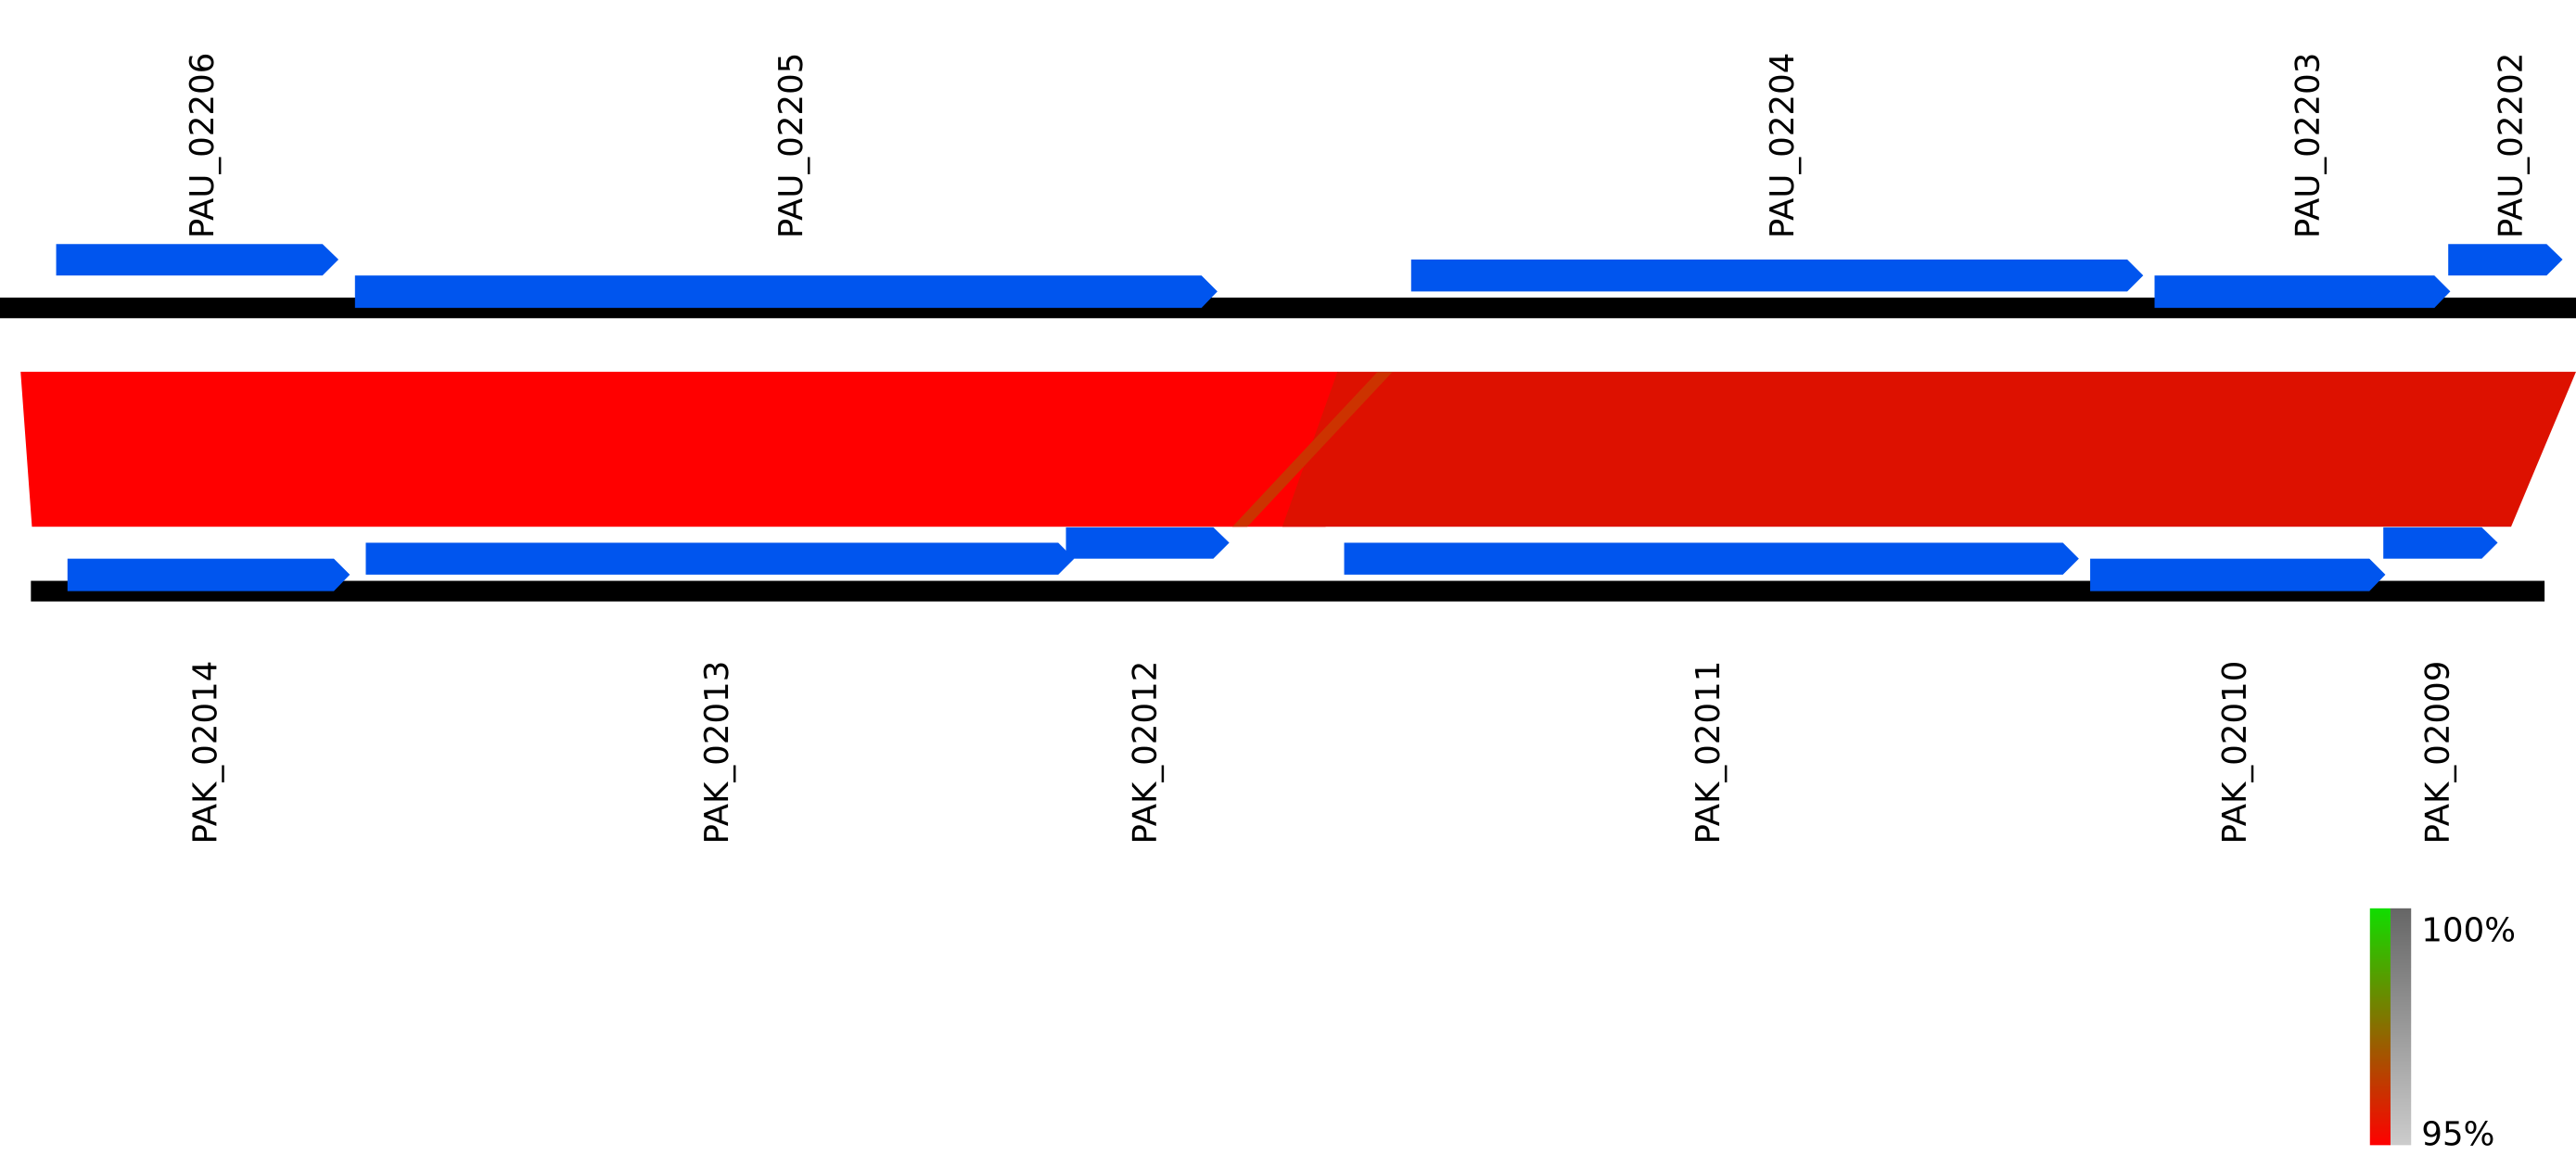
\includegraphics[width=\textwidth, trim={0 0 0 0}, clip]{/Users/joehealey/Documents/Warwick/PhD/Thesis/chapters/chapter3/img/LUMT.png}
   \put(-227,102){\customarrow{0pt}{90}}
   \put(-170,20){\small Percentage Sequence Identity}
  \end{subfigure}
  \begin{subfigure}[h]{0.9\textwidth}
   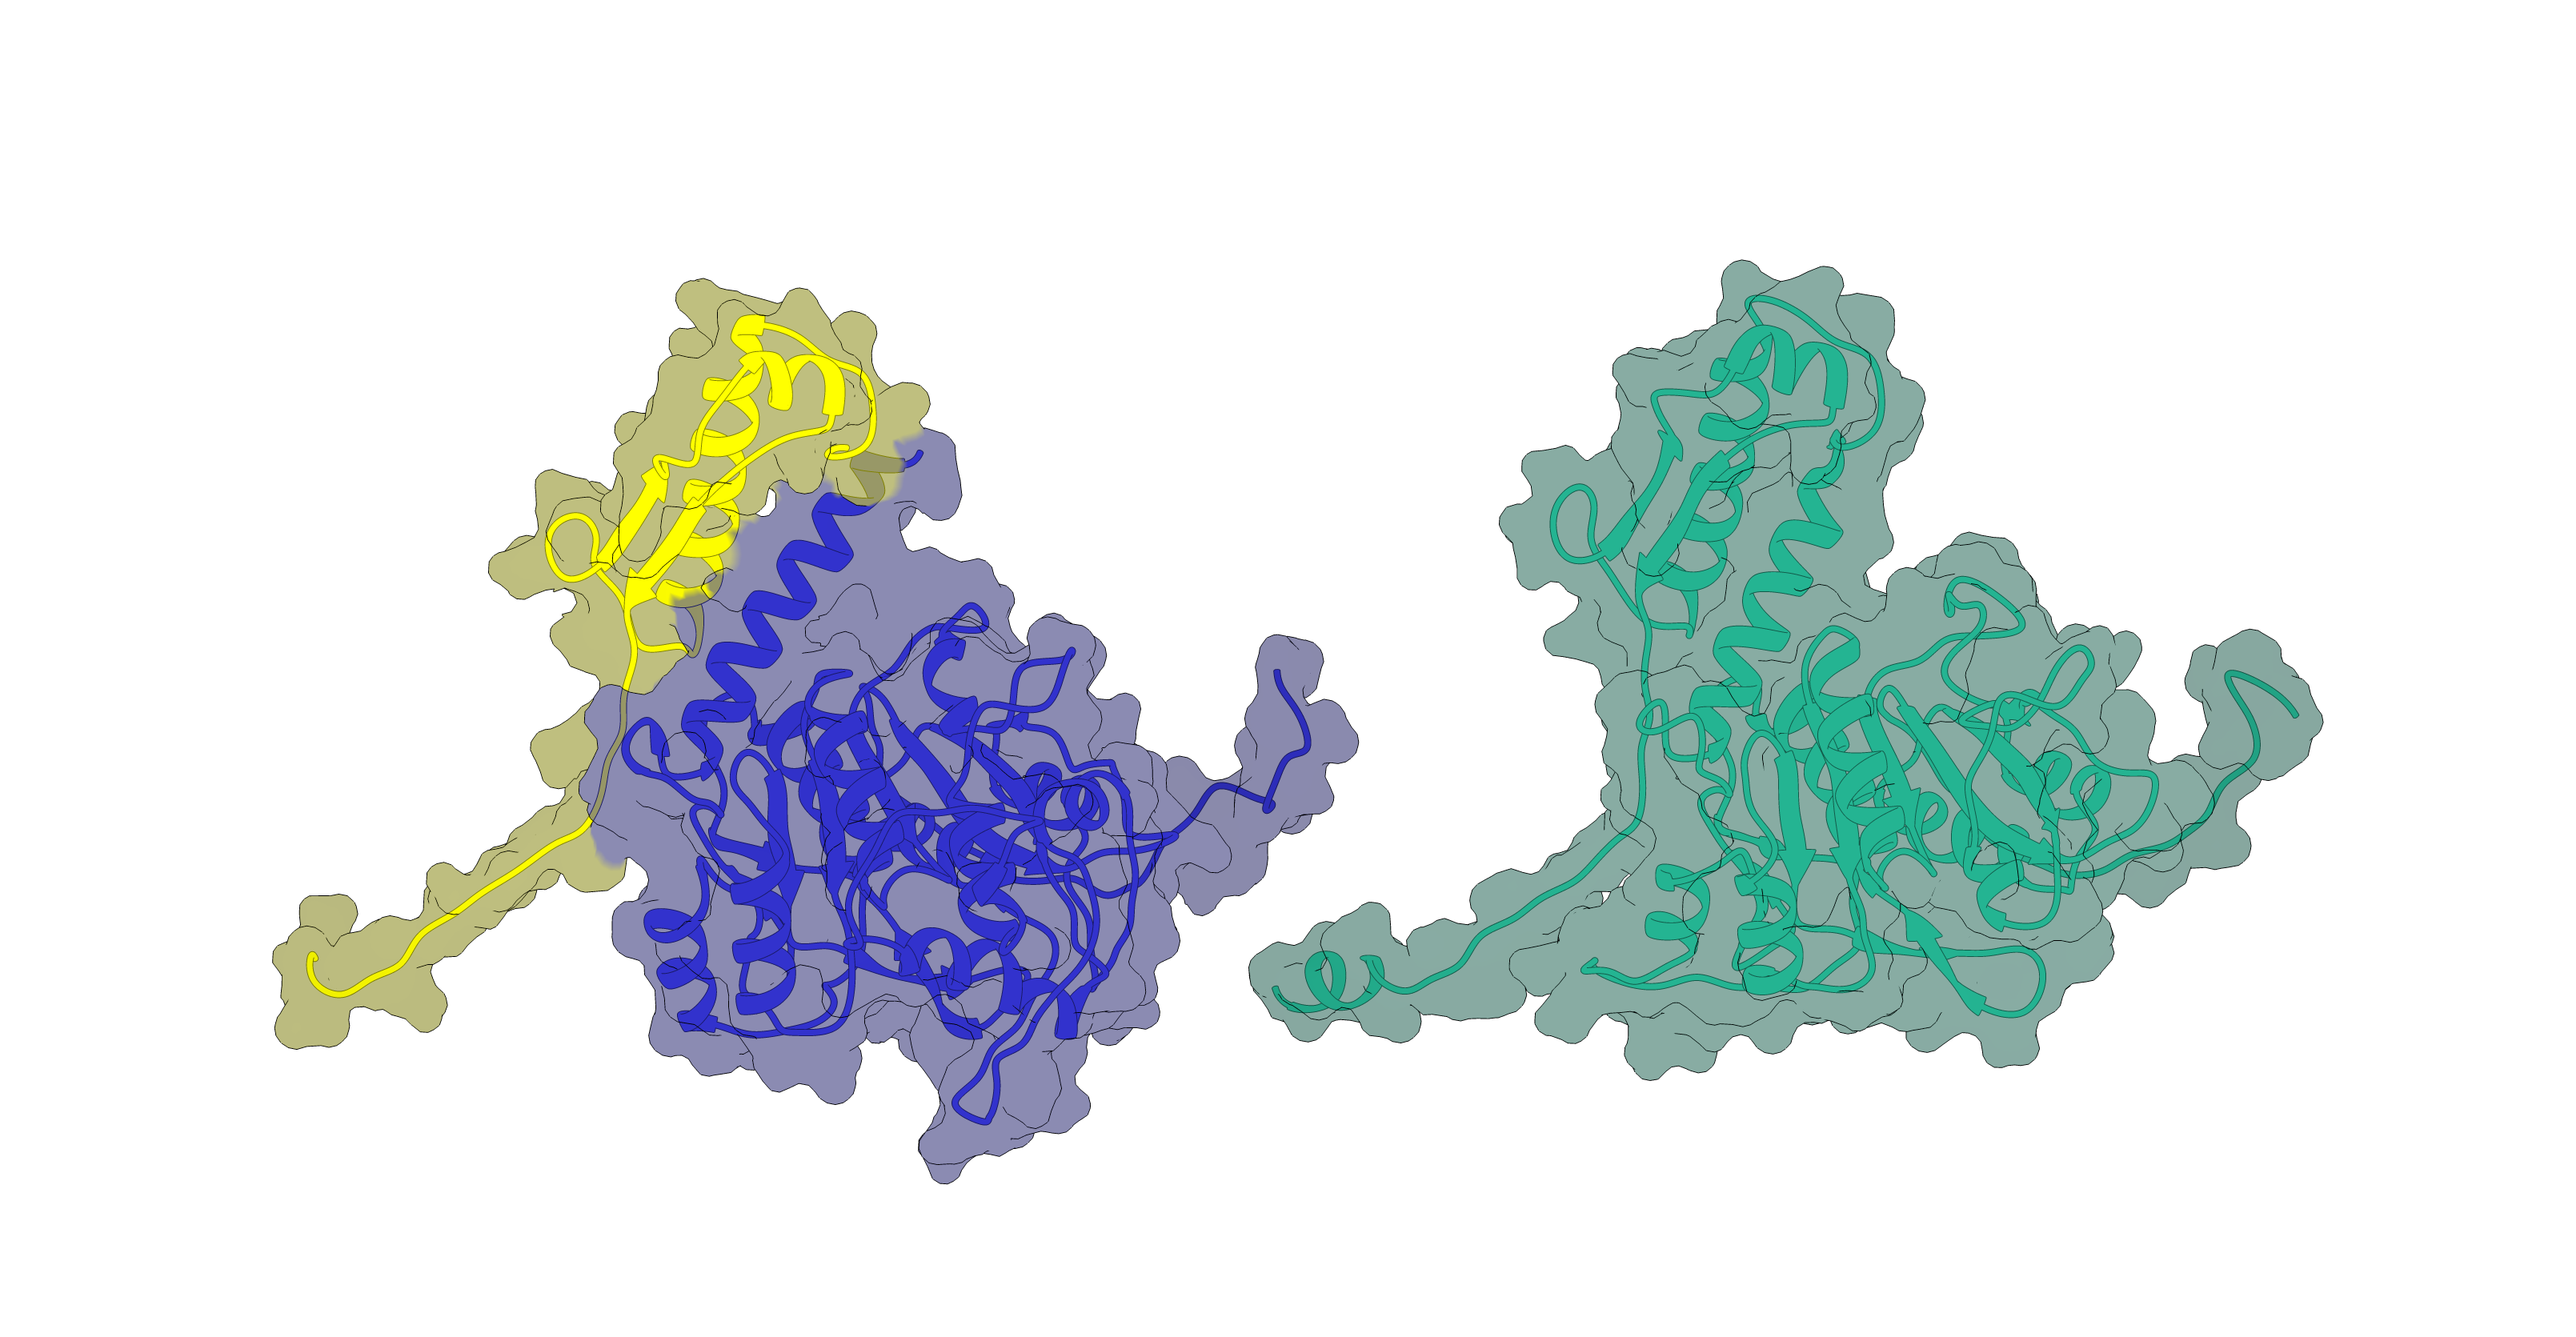
\includegraphics[width=\linewidth, trim={70 30 70 60}, clip]{/Users/joehealey/Documents/Warwick/PhD/Thesis/chapters/chapter3/img/Lumt_outersheaths.png}
   \put(-380,0){\color{Goldenrod} \textbf{PAK\_02012}}
   \put(-280,0){\color{blue} \textbf{PAK\_02013}}
   \put(-120,0){\color{Emerald} \textbf{PAK\_02011}}
   \end{subfigure}
 \captionsetup{singlelinecheck=off, justification=justified, font=footnotesize, aboveskip=10pt}
 \caption[Deletions and domain splits in the ``Lumt" operon]{\textsc{\normalsize Outer sheath proteins of PVC ``Lumt" showing a domain split.}\vspace{0.1cm} \newline The outer sheath proteins of PVC ``Lumt" from the \Pasy{} Kingscliff operon are shown. The cyan model corresponds to PVC4, an intact outer sheath protein. The dark blue model is the same model as depicted in \vref{PVC1-5_leastsimilar} in the top row for PVC2. The 2 helices that protrude from the top in other proteins are missing, instead being present as a gene split, depicted as a separate chain in yellow. The arrow in the upper alignment panel shows the gene split in in the Kingscliff ``Lumt" operon, and is compared by sequence identity to the equivalent operon in the ATCC43949 strain (just the first 6 proteins of the operon). }
 \label{lumt_outersheath}
\end{figure}


\myparagraph{Electrostatic comparisons amongst tube proteins}
There do not appear to be significant structural or fold differences that seem likely to lead to functional differences between these paralogues accounting for their maintenance. Perhaps then, the proteins may preserve their structure, but the differences brought about by diverse sequence manifest in electrostatic potentials which are in some way key to the structure of the PVCs. Given that the PVCs are proposed to carry different payload proteins with variable biophysical characteristics, there would stand to be 2 hypotheses: one, that the tube lacks any specialisation at all, allowing for many different payload to pass through, which appears to be the observed phenomenon for the T6SS \citep{Ge2015a}, or alternatively, each PVC is adapted in a particular way to its cognate payloads.

In \cite{Ge2015a}, comparisons are made regarding the electrostatics of the tube interiors, where they reason that the R-type pyocin, as a proton conducting apparatus, has a largely negative charge in order to convey such ions. Similarly, they remark that the inner sheath of the T6SS is mixed/neutral overall to cope with conveyance of diverse cargoes, and conversely that the interiors of the PS17 and $\lambda$ phages are mostly negative to convey DNA. This latter point seems as though it may be incorrect however, since the rendered, resolved, structure of the T4 tube, which conveys dsDNA, is extremely highly negatively charged - a rational for this might be a sort of `electromagnetic levitation' so that the DNA runs through the tube somewhat like a Maglev train, without `sticking' to the walls. \vref{inner_sheath_electrostatics} replicates a similar analysis for both inner tube proteins (PVC1/5), and the orthologues identified earlier (without the gp6 monomer and with PVC5 in its place however). Some potential structural differences are more apparent between PVC1 and 5 in this hexameric arrangement, but as its largely tied to loop structures, it is unadvisable to set too much store by it.


\begin{figure}[h]
 \thispagestyle{augment}
 \centering
   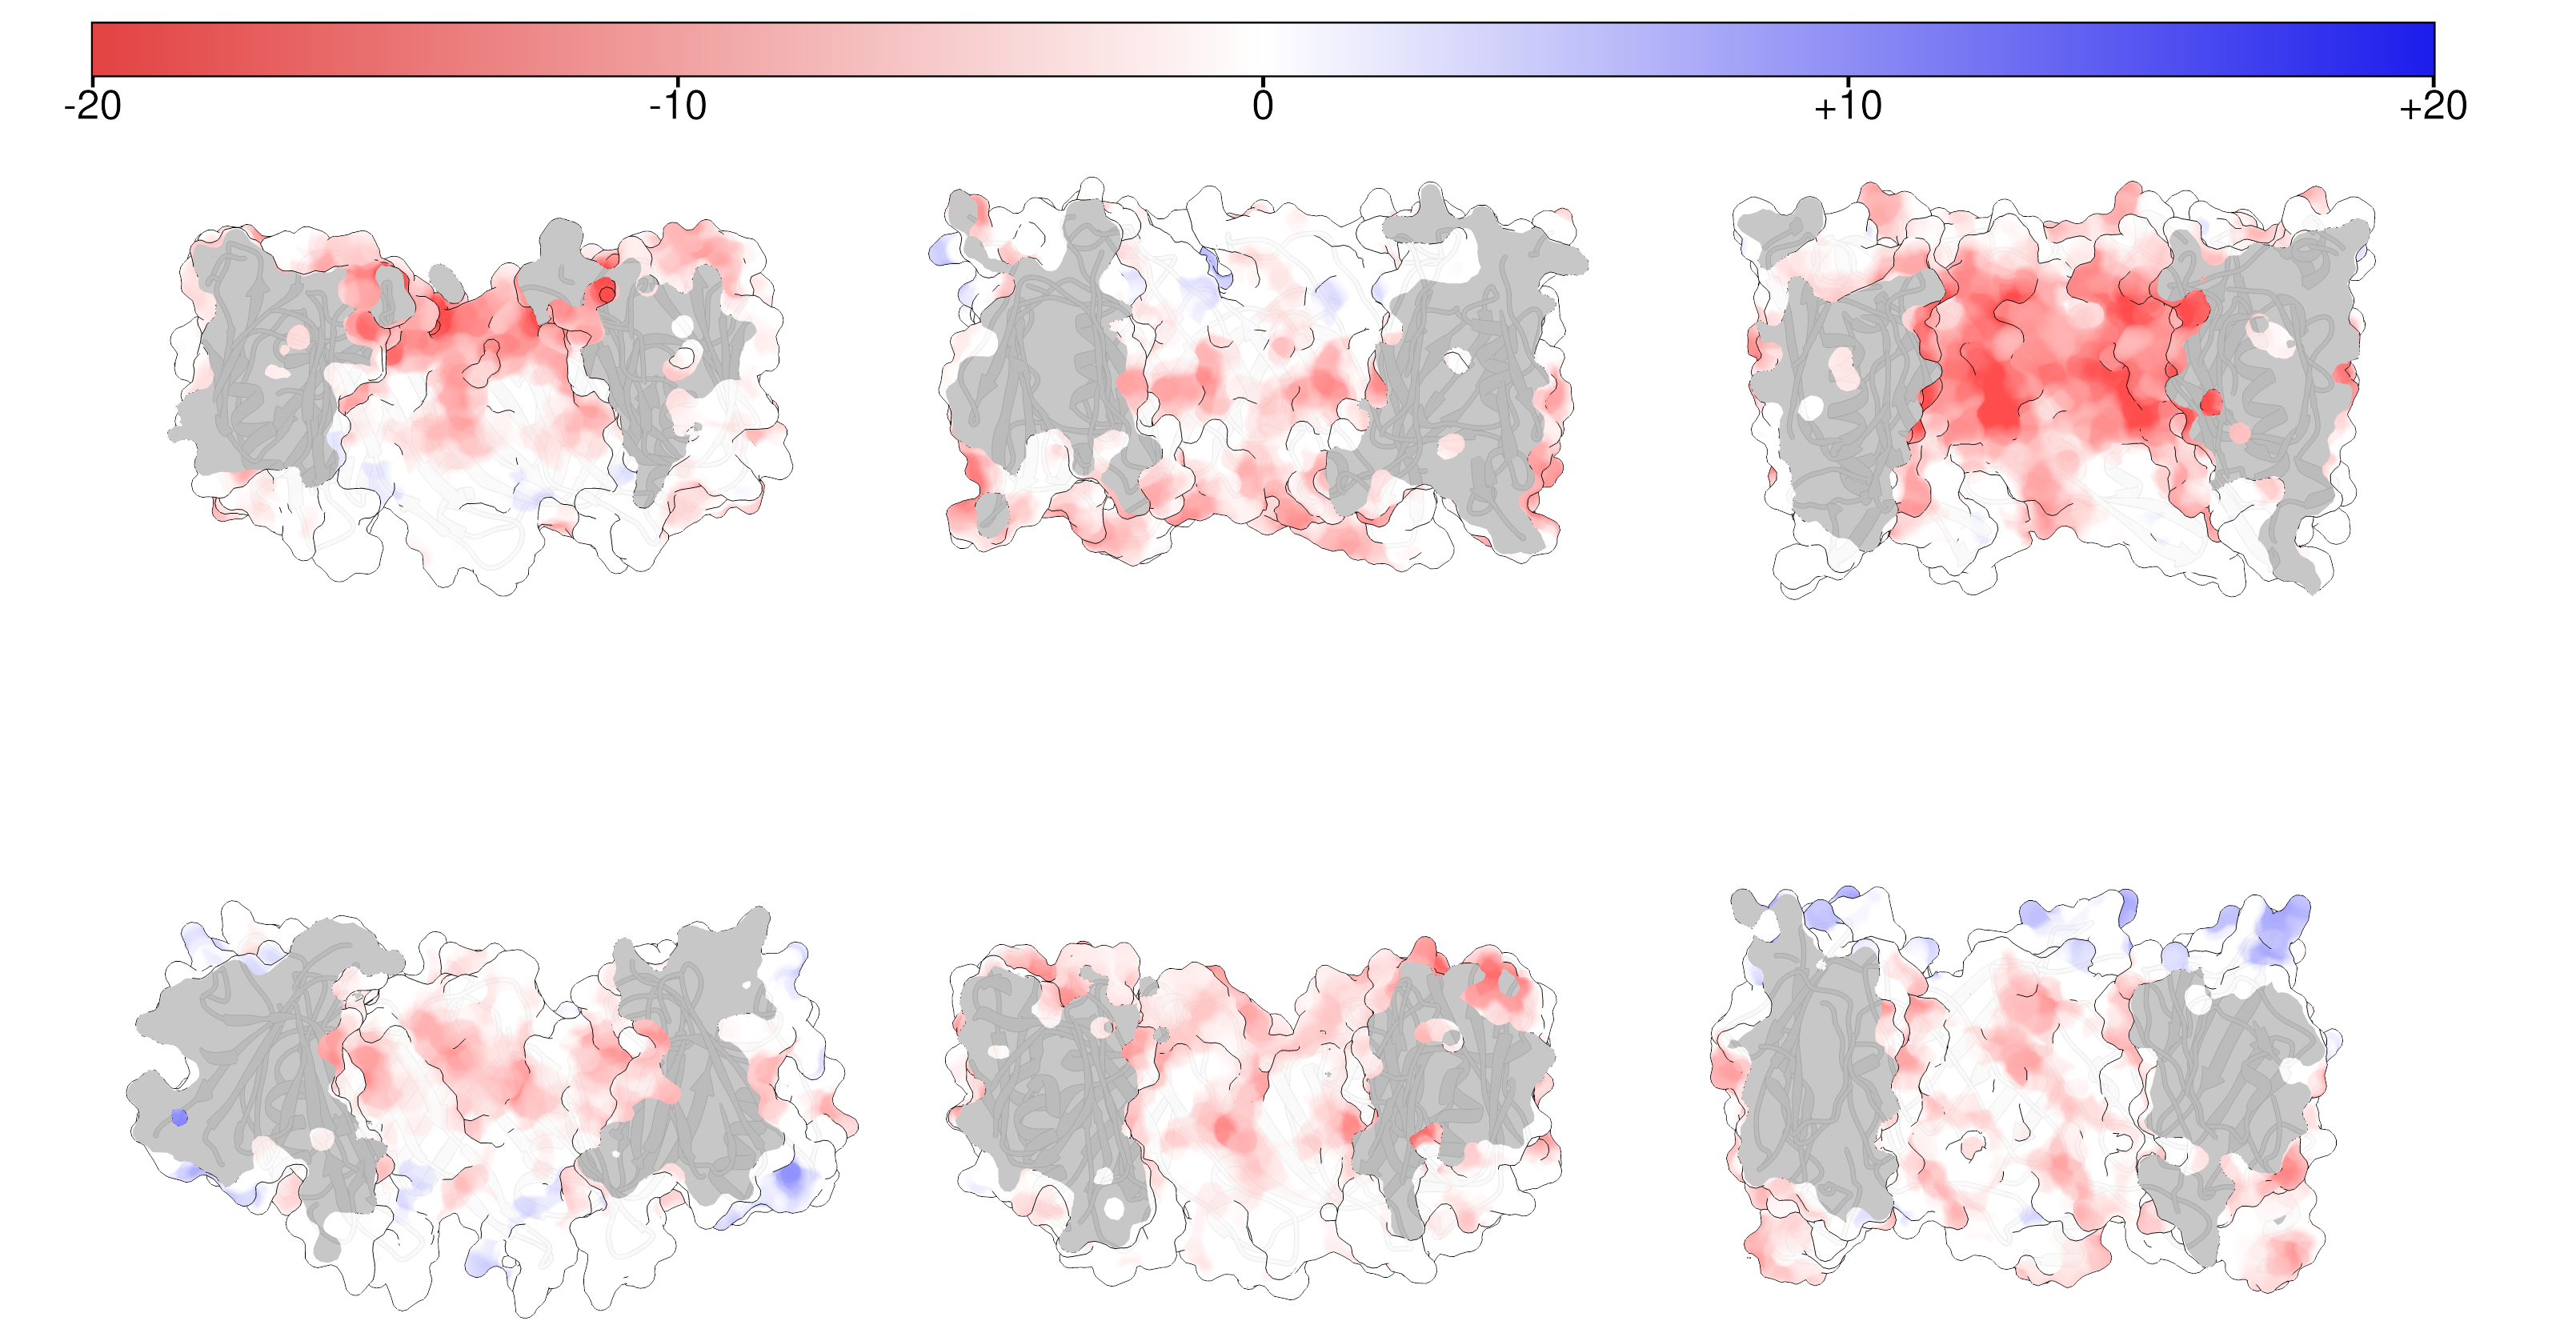
\includegraphics[width=\textwidth, trim={20 -20 20 -40}, clip]{/Users/joehealey/Documents/Warwick/PhD/Thesis/chapters/chapter3/img/Inner_tube_electrostatics.png}
   \put(-272,248){Coulombic potential}
   \put(-370,125){PVC1}
   \put(-233,125){T6SS}
   \put(-92,125){T4}
   \put(-370,0){PVC5}
   \put(-227,0){Afp}
   \put(-102,0){Pyocin}
 \captionsetup{singlelinecheck=off, justification=justified, font=footnotesize, aboveskip=10pt}
 \caption[Electrostatics of the inner sheath (cutaway)]{\textsc{\normalsize The Coulombic potentials of caudate structure inner sheaths.}\vspace{0.1cm} \newline The various inner sheath protein orthologues are rendered by their Coulombic electrostatic potential (i.e. charge), from strongly negative (dark red) through neutral (white with transparency) to strongly positive (dark blue). In consensus with the study of \cite{Ge2015a}, the R-type pyocin has a neutral to moderately negative charge in the interior. The sheath hexamers are shown as cut-aways (translucent grey faces show the `cut' path). The T6SS has mostly neutral charges (and a mixture of positives and negatives). The T4 tube appears to be overwhelmingly negatively charged, c.f. Ge et al.'s findings for the $\lambda$ and PS17 phages which were seemingly positively charged. The PVC (in both loci) and Afp, have similarly neutral-to-negative charges. In the case of PVC1, a halo of greater negative charge appears around the top, which is discussed further subsequently. The augmented reality model to accompany this figure shows the PVC1 hexamer in full 3D to give an idea of the all round electrostatics and structure.}
 \label{inner_sheath_electrostatics}
\end{figure}

Amongst all PVC1s there does not appear to be a great discrepancy in the surface potentials. All are largely negatively/neutrally charged. There are a few cases where some more prominent positive charges appear. In the case of PVC1, the exterior of the inner sheath is highly negatively charged. However, there is a prominent difference with PVC5, as it maintains a neutral and even positively charged exterior by comparison. This is surprising as it would be expected that if each monomer has to interact with an exterior sheath protein, and the sequences are largely conserved as shown previously, that both loci would carry similar charge profiles on this face.

\begin{figure}[h]
 \thispagestyle{IHA-fancy-style}
 \centering
   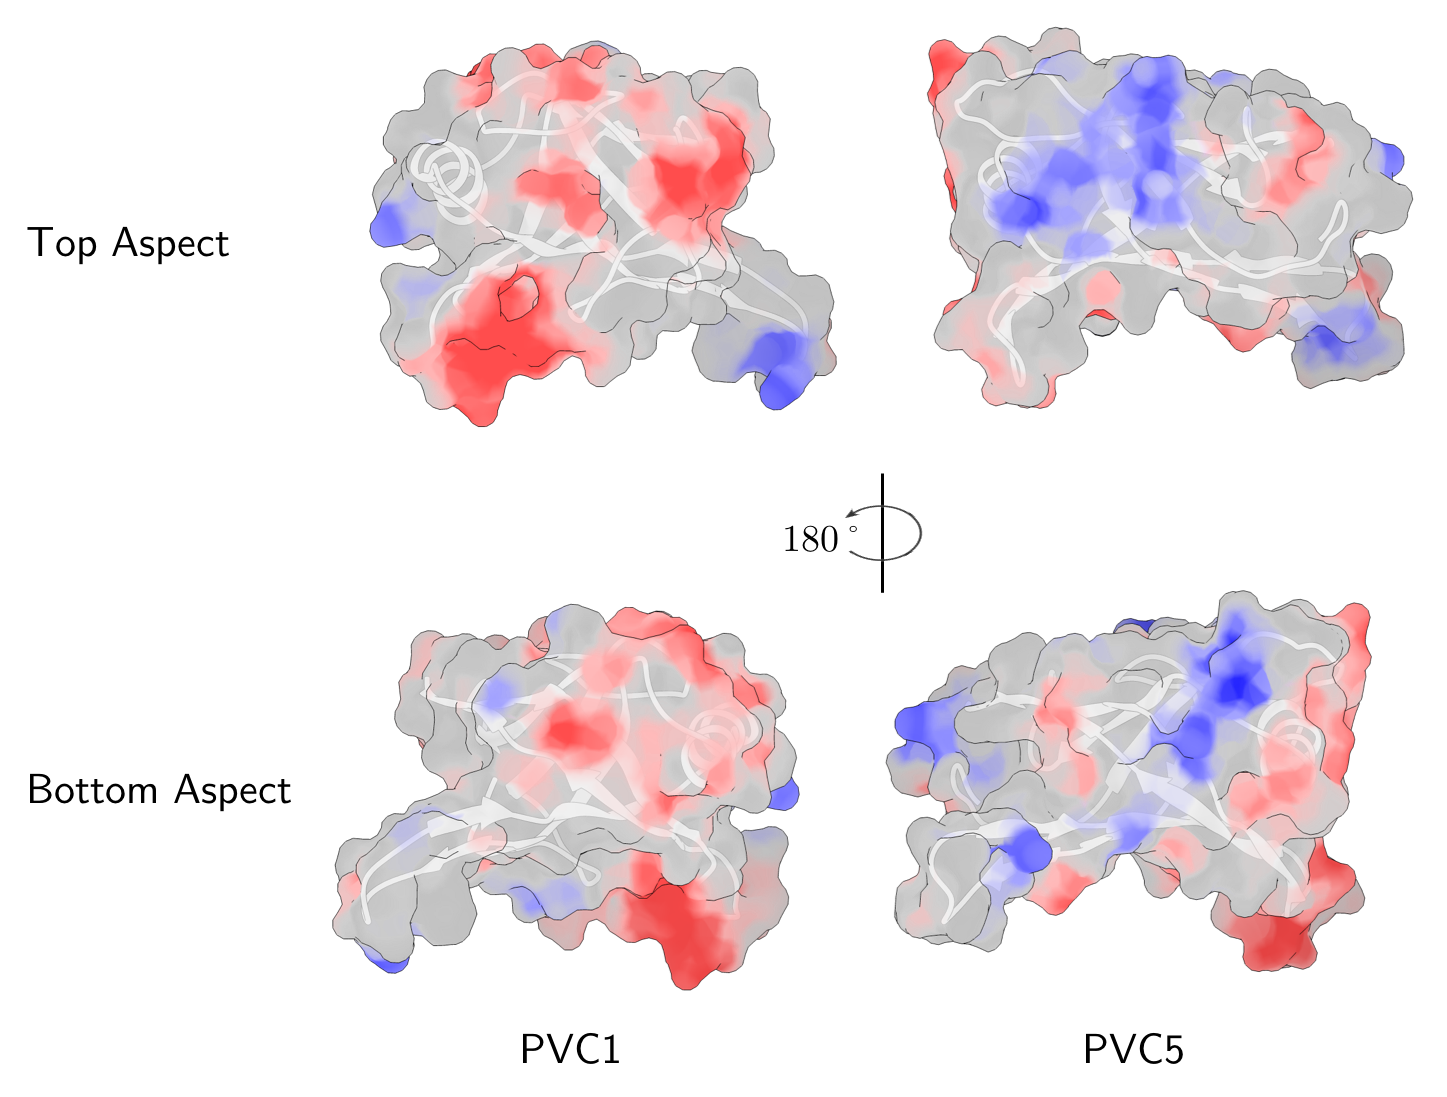
\includegraphics[width=\textwidth, trim={0 0 0 -30}, clip]{/Users/joehealey/Documents/Warwick/PhD/Thesis/chapters/chapter3/img/Pnf_top_bottom.png}
   \put(-271,318){Coulombic potential}
 \captionsetup{singlelinecheck=off, justification=justified, font=footnotesize, aboveskip=10pt}
 \caption[Electrostatic tube strata interfaces]{\textsc{\normalsize Polarities of the top and bottom faces of inner sheath monomers.}\vspace{0.1cm} \newline The electrostatic potentials of exemplar inner sheath monomers from PVC ``Pnf", loci 1 and 5. PVC1s exhibit predominantly positive charges on the `top' and `bottom' faces (the faces between disks of the tube), whilst PVC5s exhibit predominantly negative charges. This suggests that the 2 loci may form alternating hexameric stacks to assemble the tube in a directed manner like so: \texttt{(++)(--)(++)(--)}, where \texttt{(+-)} represents a monomer and its charges at either end.}
 \label{PVC1-5_charges}
\end{figure}



There seems to be further subtlety to the structural assembly of the PVCs incorporating these proteins, as the other predominant electrostatic pattern shows that PVC1 has predominantly negative charges at its `top' and `bottom', whilst PVC5 has predominantly neutral/positive charges, as demonstrated in \vref{PVC1-5_charges}. Therefore, one hypothesis is that the PVC is actually built from alternating stacks of PVC1-PVC5-PVC1-PVC5 with the negative and positive faces interacting. This is in contrast to, for example, the Pyocin tube, which has a prominent negative face, and a positive face within the same hexameric disk (visible in the bottom right of \vref{inner_sheath_electrostatics}, akin to bar magnets placed end-to-end, thus forms directionally controlled spontaneously self-assembling tube. As per the rest of the chapter so far \vref{PVC1-5_charges} shows the case for just one of the inner sheath pairs (PVC1 and 5 from PVC ``Pnf" again), but this largely holds for all 32 proteins. The side aspects of the proteins (not shown) demonstrate predominantly neutral charges, suggesting there is little significant within-disk ordering.

The outer sheath proteins remain something of a mystery. Not only is there often an additional copy of the gene, with very little obvious significant structural difference, but there does not appear to be drastic differences in charge between them. They all have predominantly neutral/positively charged interiors, but overwhelmingly negatively charged surfaces. Even with the sequence variability demonstrated in \vref{PVC1-5_conservation} and \ref{PVC1-5_leastsimilar}, there appears to have been a drive to maintain a negative overall surface charge. As an experimental indication of the models validity, an anion exchange chromatography protocol has been developed in the lab which relies on positively charged resins to retain negatively charged molecules and has worked well for purification of several PVCs to date.

As their inter- and intra-protomer interactions are more complex, \vref{PVC2-4_charges} shows a half-sheath where 3 of the 6 helical protomers have been scaffolded against the R-type pyocin's structure (a rise of 38.4 \AA, and a twist of 18.3\AA). Each protomer is made of one of the 3 paralogues from the ``Pnf" operon of ATCC43949. \cite{Ge2015a} suggest that the majority of interactions in the outer sheath are within a helical protomer, and this manifests in one of the outstretched `arms' of the outer monomers, carrying a negative charge which interacts with a positively charged groove at the neck of the monomer's two upstretched helices, below and to the left of it (as the helix is left handed).

\begin{figure}[p]
 \thisfloatpagestyle{augment}
 \centering
   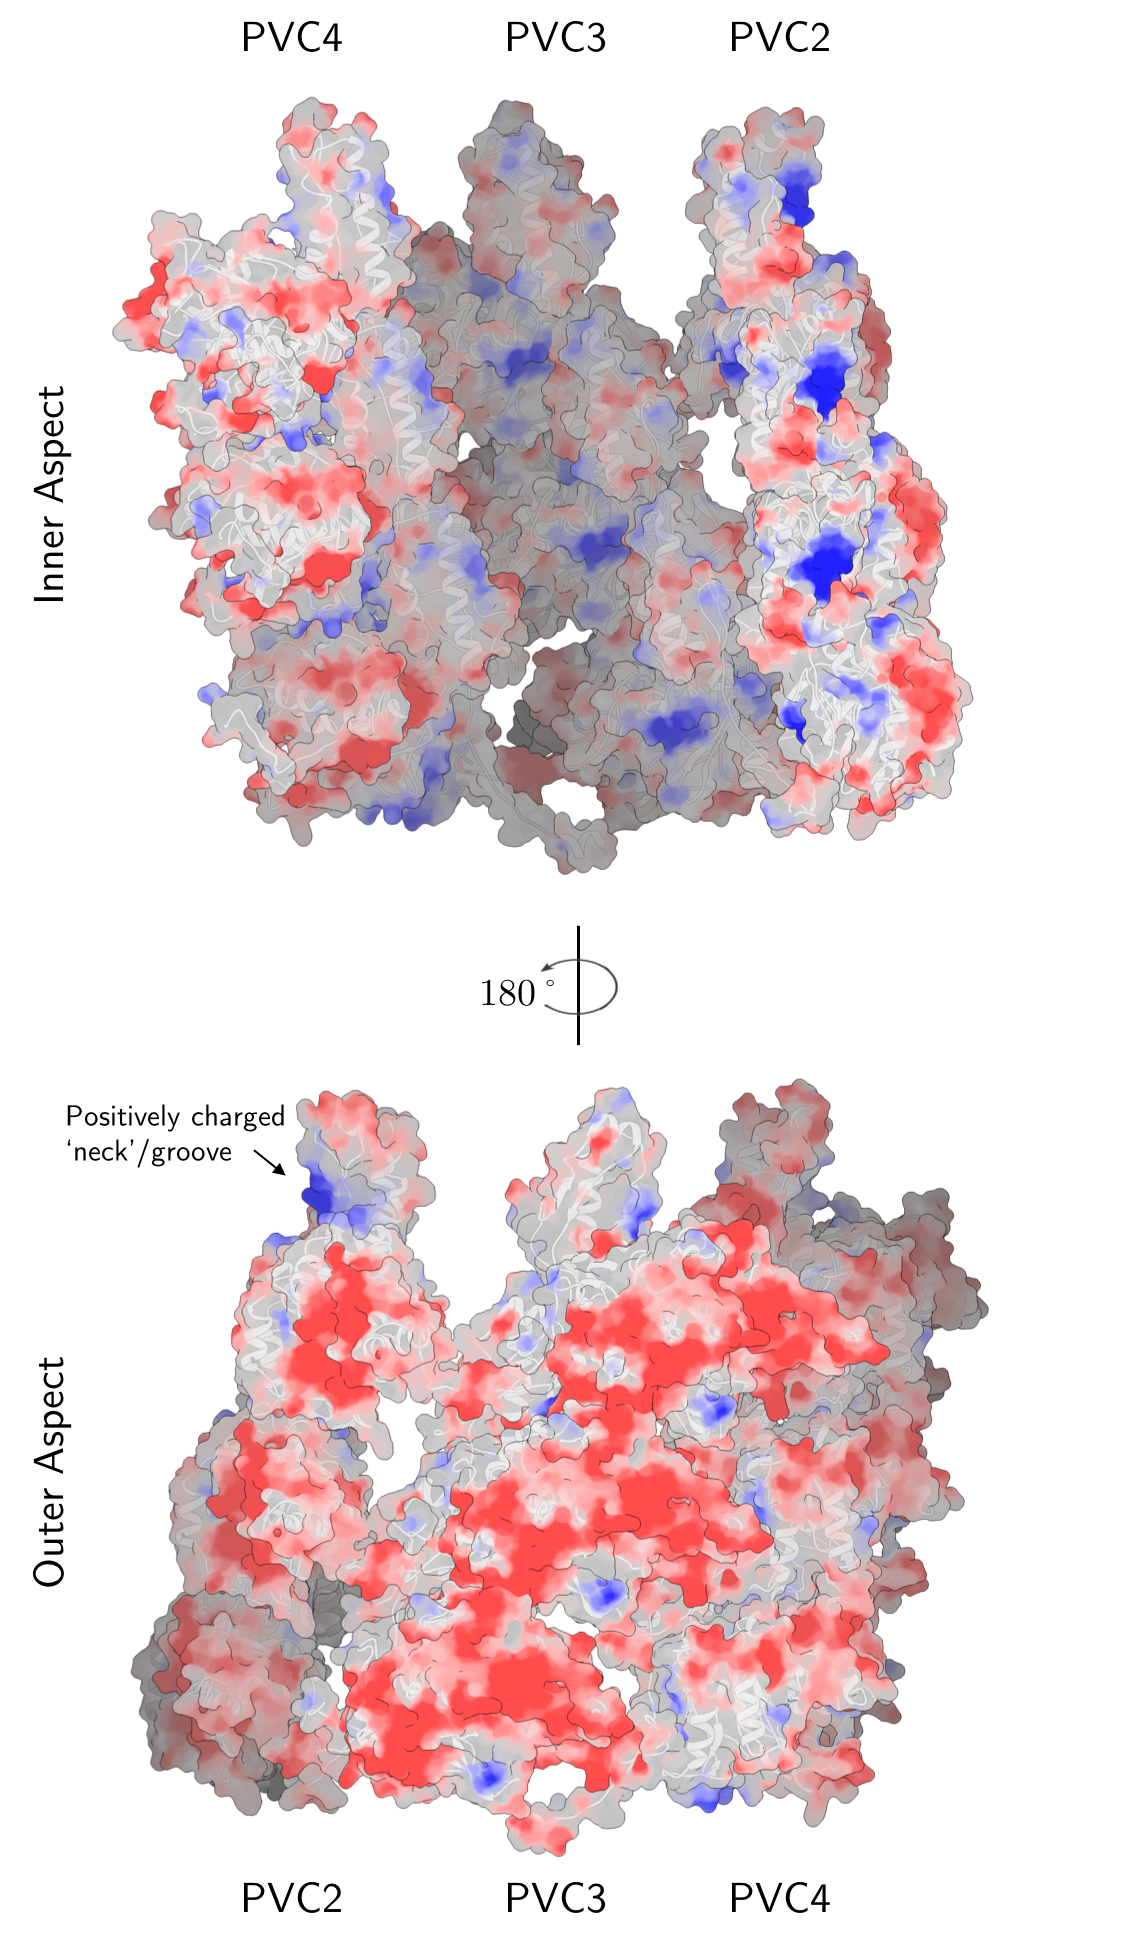
\includegraphics[width=0.81\textwidth, trim={0 0 0 0}, clip]{/Users/joehealey/Documents/Warwick/PhD/Thesis/chapters/chapter3/img/Pnf_outer_tube.png}
 \captionsetup{singlelinecheck=off, justification=justified, font=footnotesize, aboveskip=10pt}
 \caption[Electrostatic tube strata interfaces]{\textsc{\normalsize Interior and exterior aspects of outer sheath protomer electrostatics.}\vspace{0.1cm} \newline The interior and exterior of the outer sheath proteins in biologically relevant positions/conformations are shown, scaffolded positionally against the R-type pyocin tube structure (PDB ID 3J9Q). All three paralogues share similar electrostatic profiles, with the tube interface as neutral/positive, but the exterior overwhelmingly negatively charged in all cases.}
 \label{PVC2-4_charges}
\end{figure}

The most compelling alternative hypothesis, certainly for the inner sheaths, is that one of the pair is specialised as an adaptor or collar. Given that PVC5 is translationally coupled to PVC6, another putative structural protein discussed in the next section, it might be likely that this is the case for PVC5. In \vref{PVC1-5_charges}, some greater structural differences do seem to manifest when viewed as a sliced hexamer. PVC5 has a slightly `squashed' confirmation, being somewhat wider than the PVC1 hexamer, and seems to have a slightly more restricted lumen suggesting that it is perhaps less suited to comprising the bulk of the tube. This fits with legacy 2D gel proteomic analysis which found PVC1 in abundance but lower levels of PVC5, and would also fit with the Coulombic patters noticed above in that PVC5 did not demonstrate the same outer aspect potentials as PVC1 (not shown explicitly), instead being much more neutral in charge. This might make sense if the hexamer doesn't have to interact with the outer sheath proteins like PVC1 might. \vref{PVCvsT4} shows a colour coded, stripped down, T4 baseplate complex, demonstrating that there are 2 additional proteins, gp48 and gp54 (red/orange), which form a transition between the inner tube and the spike, and resemble subtly modified inner sheath proteins. Interestingly, HHPred fails to attribute this orthology, instead matching primarily to the tube proteins themselves which may also have influence the homology modelling process. The figure shows the bulk of the baseplate hub in monochrome shades, the tube in yellow, and 2 fitted PVC proteins as white surface models. Outer sheath proteins are not shown.

Better RMSDs are obtained when matching PVC5 to gp54, than to gp48, so it is unclear whether there is another protein which fulfils the role of gp48 or whether PVCs have a simplified baseplate; certainly, their baseplates lack the vast majority of peripheral T4 baseplate proteins (which are omitted from the figure but the extent can be seen in the EM map).

\begin{figure}[p]
 \thisfloatpagestyle{augment}
 \centering
   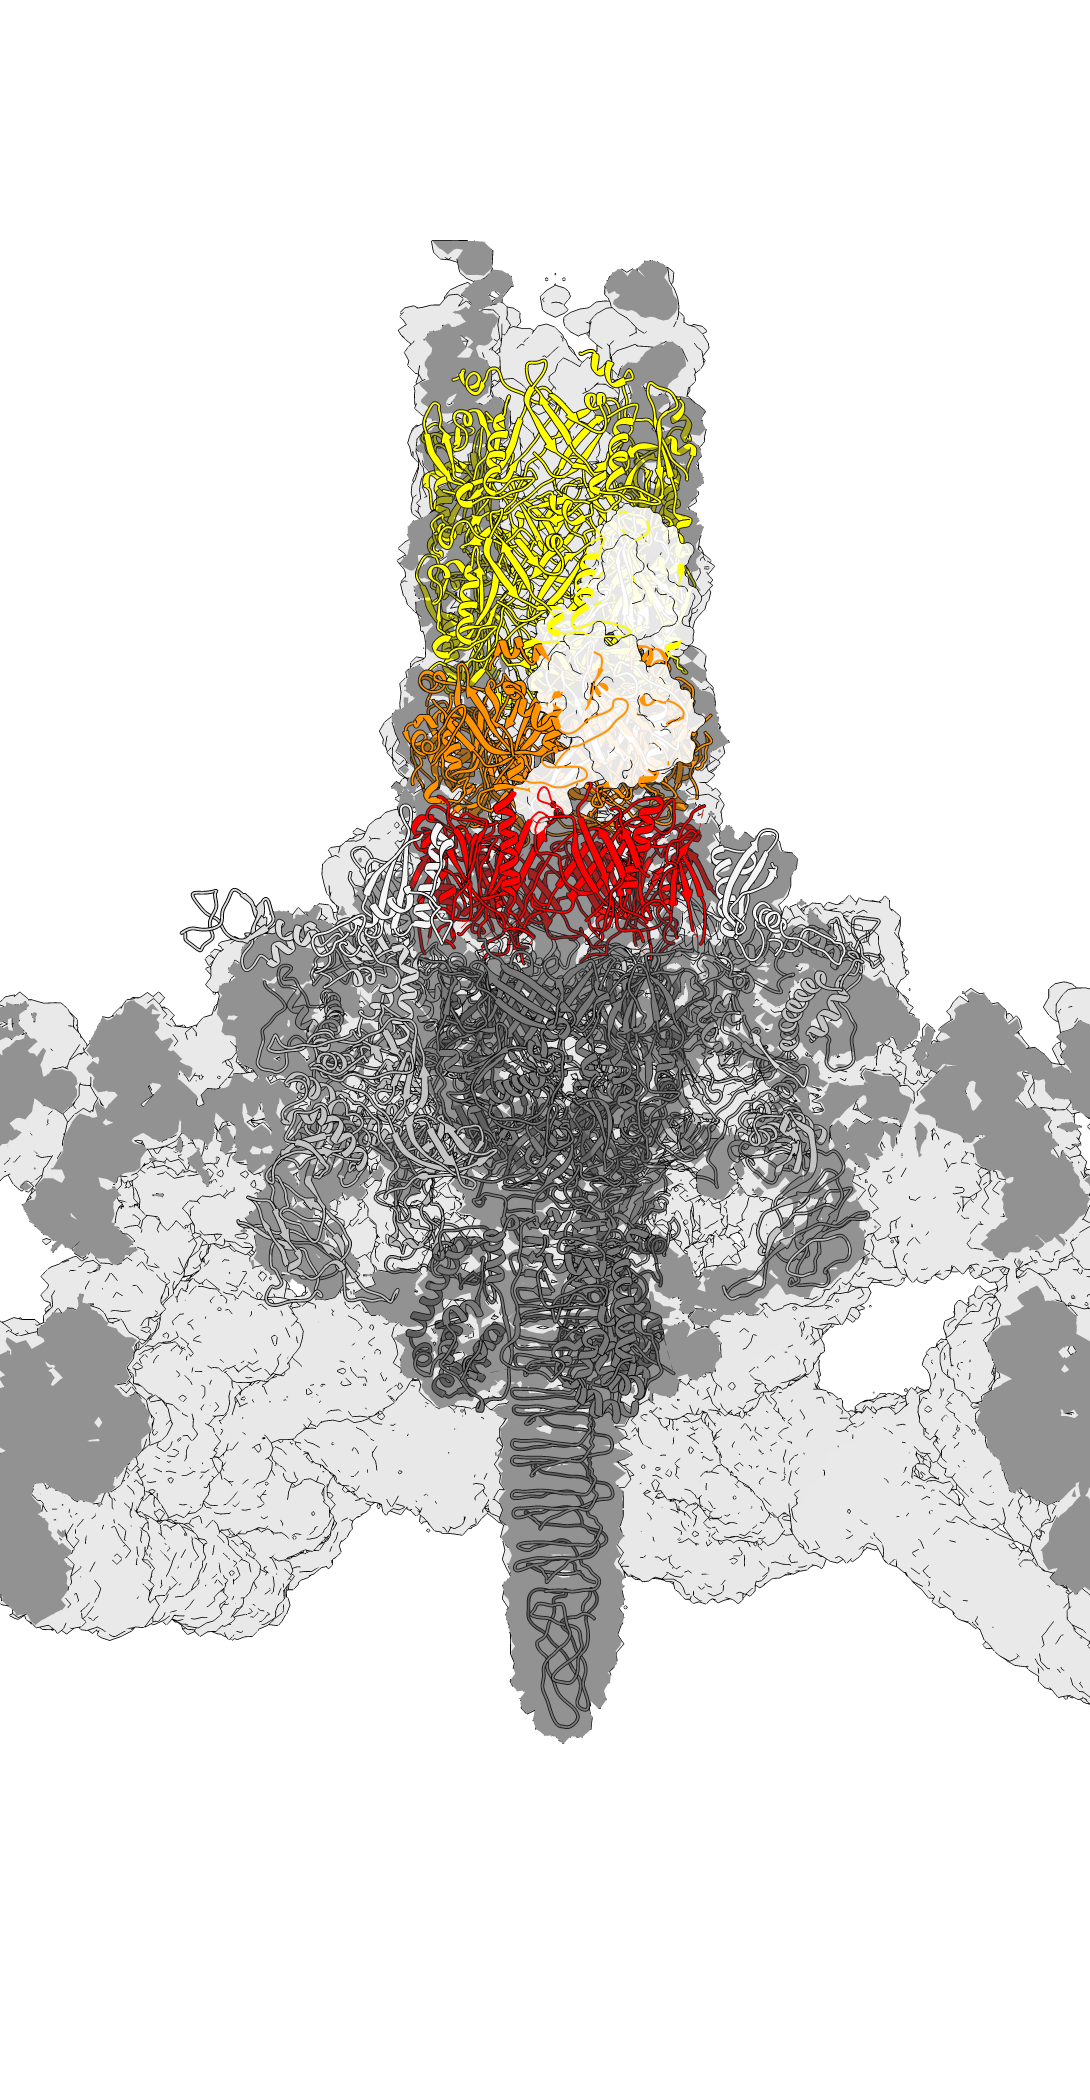
\includegraphics[width=\textwidth, trim={0 80 0 55}, clip]{/Users/joehealey/Documents/Warwick/PhD/Thesis/chapters/chapter3/img/PVC5_in_T4.png}
   \put(-130,460){\customarrow{-1pt}{0} gp19 / PVC1}
   \put(-135,410){\customarrow{-1pt}{0} gp54 / PVC5?}
   \put(-137,377){\customarrow{-5pt}{35} gp48 / PVC5?}
 \captionsetup{singlelinecheck=off, justification=justified, font=footnotesize, aboveskip=10pt}
 \caption[Comparisons of PVC5 to the collar components of the T4 phage]{\textsc{\normalsize Colour coded T4 baseplate collar proteins compared to PVC subunits.}\vspace{0.1cm} \newline The baseplate hub and collar of the inner tube for the T4 bacteriophage (PDB ID 5IV5 and EMDB 3374) are shown colour coded to identify the adaptor proteins that interface the spike complex (monochrome) with the tube (yellow). This chapter proposes that PVC5 is not actually a tube monomer, but instead may form one of these 2 strata of adapters in a simplified complex.}
 \label{PVCvsT4}
\end{figure}



\clearpage
\subsubsection{The spike complex}
\begin{figure}[h!]
\thisfloatpagestyle{IHA-fancy-style}
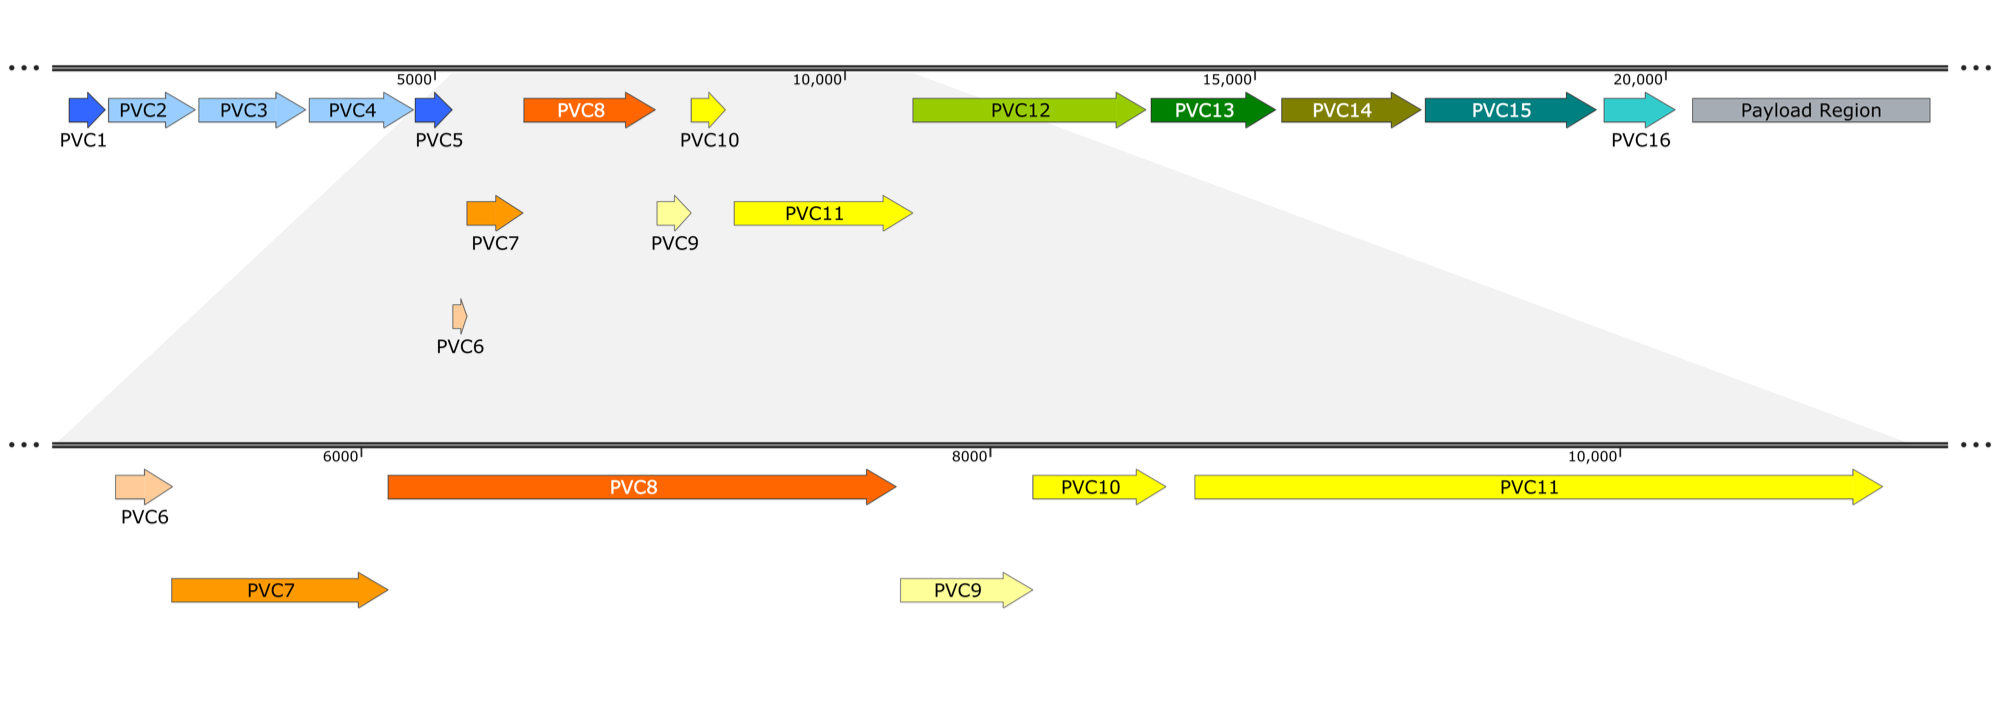
\includegraphics[width=\linewidth]{/Users/joehealey/Documents/Warwick/PhD/Thesis/chapters/chapter3/img/PVC6-11_expanded_map.png}
	\captionsetup{singlelinecheck=off, justification=justified, font=footnotesize, aboveskip=10pt}
	\caption[Spike complex protein region of a PVC operon]{\textsc{\normalsize The 6 loci predicted to comprise the spike and baseplate complex of a PVC.}\vspace{0.1cm} \newline The Pnf operon is used as an exemplar of the numbering of loci within an archetypal PVC operon, and 3 colourings are used to demarcate the `functional units' of an operon: blue - tube proteins, orange/yellow - spike complex proteins, green/cyan - the operon `core'. The 5 loci that give rise to the functional unit of the spike complex itself are blown up below as an aid to understanding the operon organisation and the proteins under discussion.}
	\label{PVC6-10map}
\end{figure}

The next 5 genes are a mixture of well resolved structures and complete enigmas. The most prominent gene in this cluster is PVC8, a VgrG/gp27-5 orthologue which is proposed to form the membrane puncturing spike at the tip of the tube. A complex of miscellaneous baseplate proteins and the spike itself are proposed to be a kind of `nucleation' site for the initial assembly of the tube. Given their syntenic position and the fact that several of the genes are translationally coupled, it seems likely that they may all have roles in the structural basis of the tube, likely within a collective collar/baseplate. PVC6 is actually translationally coupled to PVC5 in the `tube unit' of the operon, but without any good orthologies to suggest possible functions, the best hypothesis is that it may form an adapter or collar protein which interfaces the inner tube with the spike protein, since there is a transition at this interface from the 6-fold symmetry of the tube, to 3-fold in the spike complex.

A number of the (extremely weak) orthologies detected for PVC loci 6 and 7 seem to suggest enzymatic domains so it may be the case that these proteins are involved in the assembly of the PVC, but not in the structure itself.
\clearpage
\scriptsize
\rowcolors{2}{gray!10}{white}
\begin{tabularx}{\textwidth}{
>{\centering\arraybackslash} m{0.11\textwidth}
>{\centering\arraybackslash} m{0.11\textwidth}
>{\raggedright\arraybackslash} X
>{\raggedright\arraybackslash} X
}
\hiderowcolors
\captionsetup{singlelinecheck=off, justification=justified, font=footnotesize, belowskip=5pt}
\caption[HHPred hit summary for PVC6-10]{\textsc{\normalsize HHPred orthology summary for the putative baseplate and spike complex.}\vspace{0.1cm} \newline A summary of homology matches via HHPred for PVC loci 6-10. They represent a `collapsed' set of common or plausible hits from all the variants for each locus. Many of the loci in this section of the operon have poor orthologies detected. PVC8 and 9 are the only proteins with high scoring orthologies detected. All scores for the most recent analysis can be found in Appendix \vref{structural_appendix}.}\\
\label{tubehomologs}\\
Locus & PDB ID Hit & Structure & Component \\
\hline\hline
\showrowcolors
\hline

PVC6  &  Various & Various & Assorted enzymes/kinases (?)     \\
PVC7  &  5A3A    & n/a     & SIR2 Family metalloprotease (?)  \\
PVC8  &  2P5Z    & T6SS    & VgrG                             \\
PVC9  &  2IA7    & T4      & Tail lysozyme                    \\
PVC10 &  4JIV    & T6SS    & PAAR-spike tip (?)               \\
PVC11 &  3H2T    & T4      & Baseplate structural protein gp6 \\
\end{tabularx}
\hrule
\vspace{0.1cm}
{\tiny \noindent (?) denotes common or potentially plausible hits with very weak scores.}
\normalsize


Proceeding in turn, PVC6 demonstrates no reliable orthologies whatsoever. Even with the more sensitive approach of using HMMs, the lowest E-value obtained for a hit is $>$1. The only potentially informative information available is that the proteins are all quite short, at only $\approx$61 amino acids, and the structural simulations resulted, almost universally, in a pseudo-L-shaped helix-turn-helix structure, with a degenerate position forming the start of the turn (all structures not shown for brevity). While this doesn't provide information much to go on, it may suggest that this protein forms an augmentation to another structural protein, or perhaps forms a kind of lynchpin to lock elements of the structure together, given its size and potentially simple shape.


In the case of PVC7, the hits are mixed, but dominated by matches (albeit weak ones) to an SIR2 family ADP-Ribsosyltransferase from \emph{Streptococcus pyogenes} \citep{Shore2000}, with the next most plausible hit being to an EssC-like chaperone of the \emph{Pseudomonas} Type 3 Secretion System \citep{Vogelaar2010}. While again, drawing too many conclusions from such weak similarities is unadvisable, it may be the case that these hits indicate that PVC7 has a role in assembly rather than the structure itself, potentially though some enzymatic or chaperone-like mechanism. Since the structural proteins are typically identifiable through structural homology, it is possible that PVC7 does not contribute directly to the structure proper. It is a much larger protein therefore the models simulated are likely among the more spurious, and they do indeed have some of the larger RMSDs to even the closest HMM matches (on the order of $\approx$20 \AA). Unfortunately, both PVC6 and 7 remain a mystery, and are therefore prime candidates for structural resolution and mutagenesis studies.

This chapter proposes the idea that this section of the operon is made up of proteins which contribute to a baseplate and spike complex in some form or other. This may not be the case for the enigmatic PVC6 and 7, but almost certainly is for PVC8 and 9, and potentially 10. Firstly, PVC8 has long been identifiable as a structural orthologue of the VgrG class of trimeric `spikes' which sit atop the inner tubes of every caudate structure identified to date. In T4, this spike is comprised of gp27 which forms a sort of trimeric adapter which interfaces with the hexameric tube, bridging the difference in symmetry. As mentioned in \vref{introduction}, VgrG's can be decorated with many additional functional domains (also forming toxins in their own right in some cases). The models obtained here indicate that PVCs employ a simplified spike complex, closer in structure to a T6SS like that of uropathogenic \emph{E. coli} \citep{Leiman2009}.

\begin{figure}[p]
 \thisfloatpagestyle{augment}
 \centering
 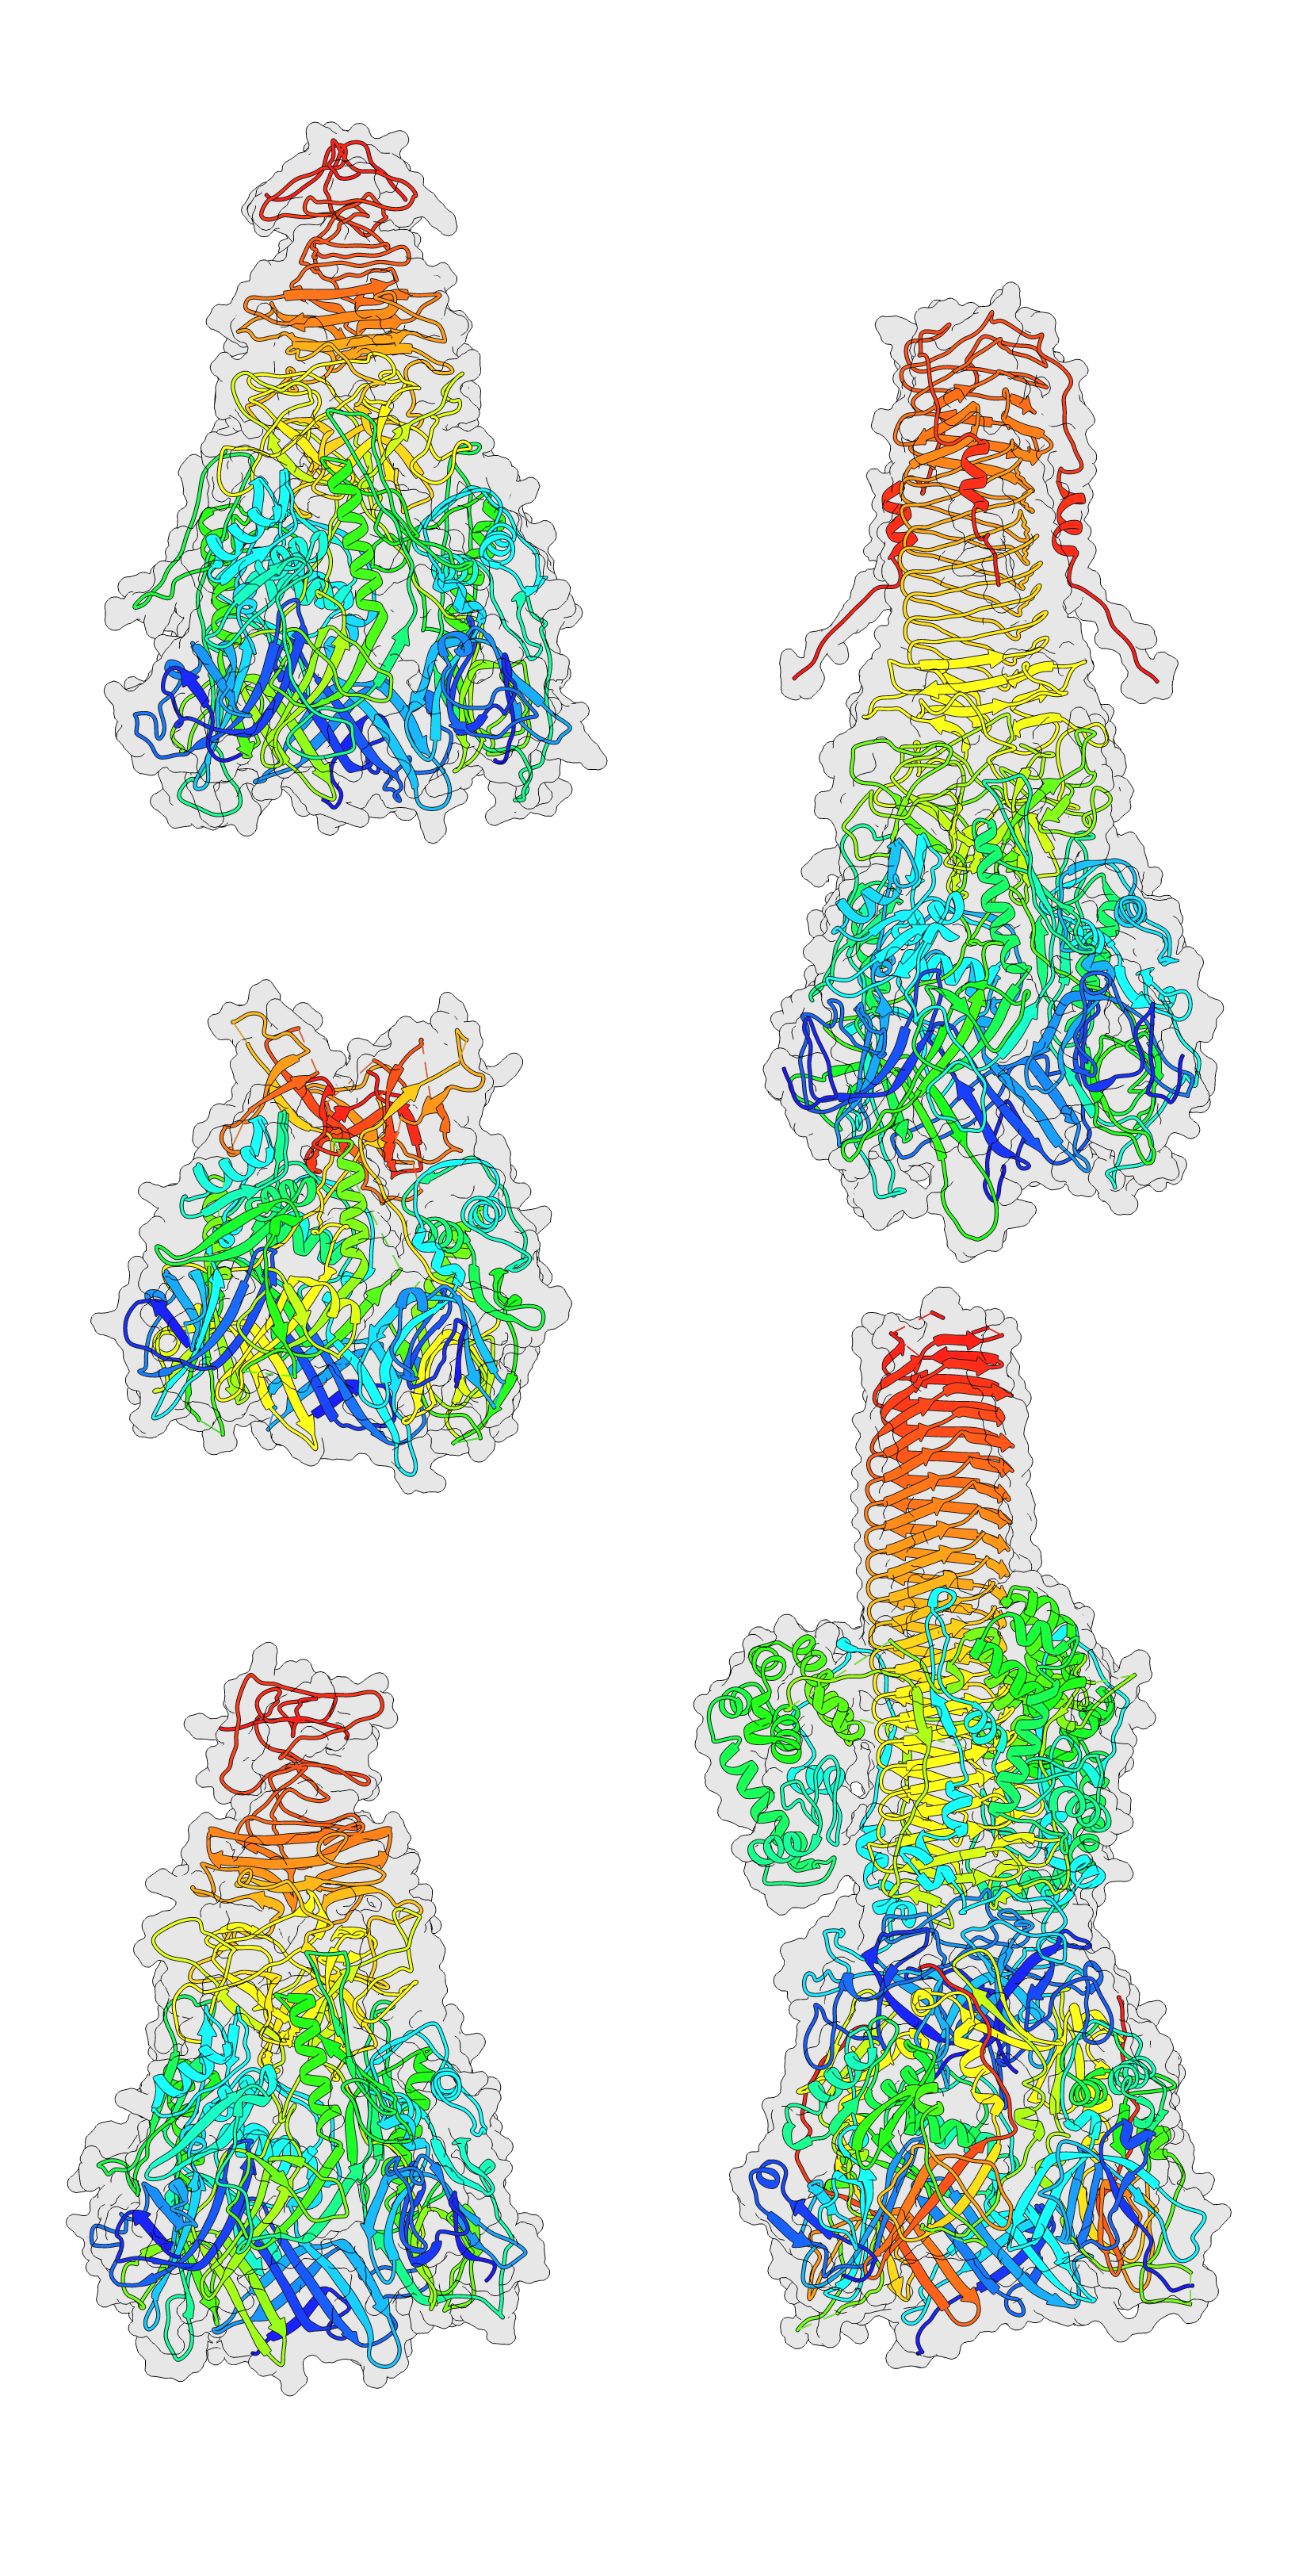
\includegraphics[width=0.75\textwidth, trim={0 0 0 0}, clip]{/Users/joehealey/Documents/Warwick/PhD/Thesis/chapters/chapter3/img/spikes.png}
 \captionsetup{singlelinecheck=off, justification=justified, font=footnotesize, aboveskip=10pt}
 \put(-265,400){PVC}
 \put(-280,240){T6SS (UPEC)}
 \put(-265,10){Afp}
 \put(-110,350){T6SS (\emph{Pseudomonas})}
 \put(-75,10){T4}
\caption[PVC8 is the major spike complex of a PVC]{\textsc{\normalsize The PVC8 spike complex compared with homologues from T4, T6SS and Afp.}\vspace{0.1cm} \newline As one of the most distinctive proteins in the operon, annotations for this protein have proven reliable, however VrgG-like spikes are well known in the literature to be variable and share little sequence similarity. PVC spikes appear more like a simplified T6SS than like T4.}
	\label{spike}
\end{figure}


Particularly prominent appears to be the loss (in the non-T4 complexes) of the `wings' that the T4 spike exhibits, flanking the extended ``$\beta$-prism". \cite{Kanamaru2002a} identified these as tail spike lysozyme domains of the gp5 protein, which T4 is proposed to use to `chew through' the peptidoglycan cell wall of target bacterial cells. With no cell wall to negotiate in eukaryotic targets, it stands to reason that the T6SS, PVCs and Afps have lost this (though the T6SS does mediate prokaryotic interactions as well, so may have other mechanisms/orthologues it can substitute in to solve this problem). In T4, the structure is comprised of 2 separate proteins, gp27, which forms the `OB-fold' at the base of the structure and gp5 which contains the lyosozyme domain and forms the prominent $\beta$-prism at the very apex of the spike. In the simulations for the PVC and Afp, this upper prism area is less well defined, and in the case of the crystallised VgrG from the uropathogenic \emph{E. coli}, it has failed to be crystallised/resolved. Based purely on protein chain length however, it does appear that the stretch of prism in the PVCs and Afps might be shorter. As a further example of the sequence variability and apparent potential for drift or adaptation of the VgrG-like spikes, the distance between the PVC and Afp orthologues is comparatively higher than for other loci studied so far, even with very similar tertiary structures among orthologues. 

\clearpage
PVC9 has also been identified by sequence searches and annotation, as an orthologue of the PDB ID 2IA7, which has been listed as a putative tail lysozyme. This has always been a point of some confusion though, as it is not clear what role a lysozyme would have in the biology of PVCs, since they have never demonstrated any antimicrobial activity. With the loss of the gp5-like lysozyme domain in the PVC8/VgrG/gp27-5 orthology locus, it seemed that this might present a domain split, and that this domain had moved to a locus of its own. Nevertheless, with no cell wall to act upon in anti-eukaryotic virulence, the only other hypothesis proposed was that this may be a mechanism of release for the PVCs, by degrading the host bacterium cell wall. This also seemed some what unlikely, since the locus is carried squarely within many other putatively structural proteins.

On inspecting the structures, PVC9 candidates do indeed closely resemble the best HMM hit, PDB ID 2IA7, a putative tail lysozyme from \emph{Geobacter sulfurreducens}. However, they also closely structurally match the gp25 baseplate initiator protein of the T4 bacteriophage (PDB ID 5IW9), even though the E-value for this match (whilst still good) is 3 orders of magnitude greater. \vref{initiator} demonstrates the similarity between an example PVC9, the \emph{G. sulfurreducens} structure, and gp25 of T4 in purple, blue and orange respectively. The RMSD between the putative lysozyme and the example PVC9 used is 1.2\AA, whilst between PVC9 and the gp25 PDB ID 5IW9 is is less than 0.3\AA.

\begin{figure}[h]
\thispagestyle{IHA-fancy-style}
\centering
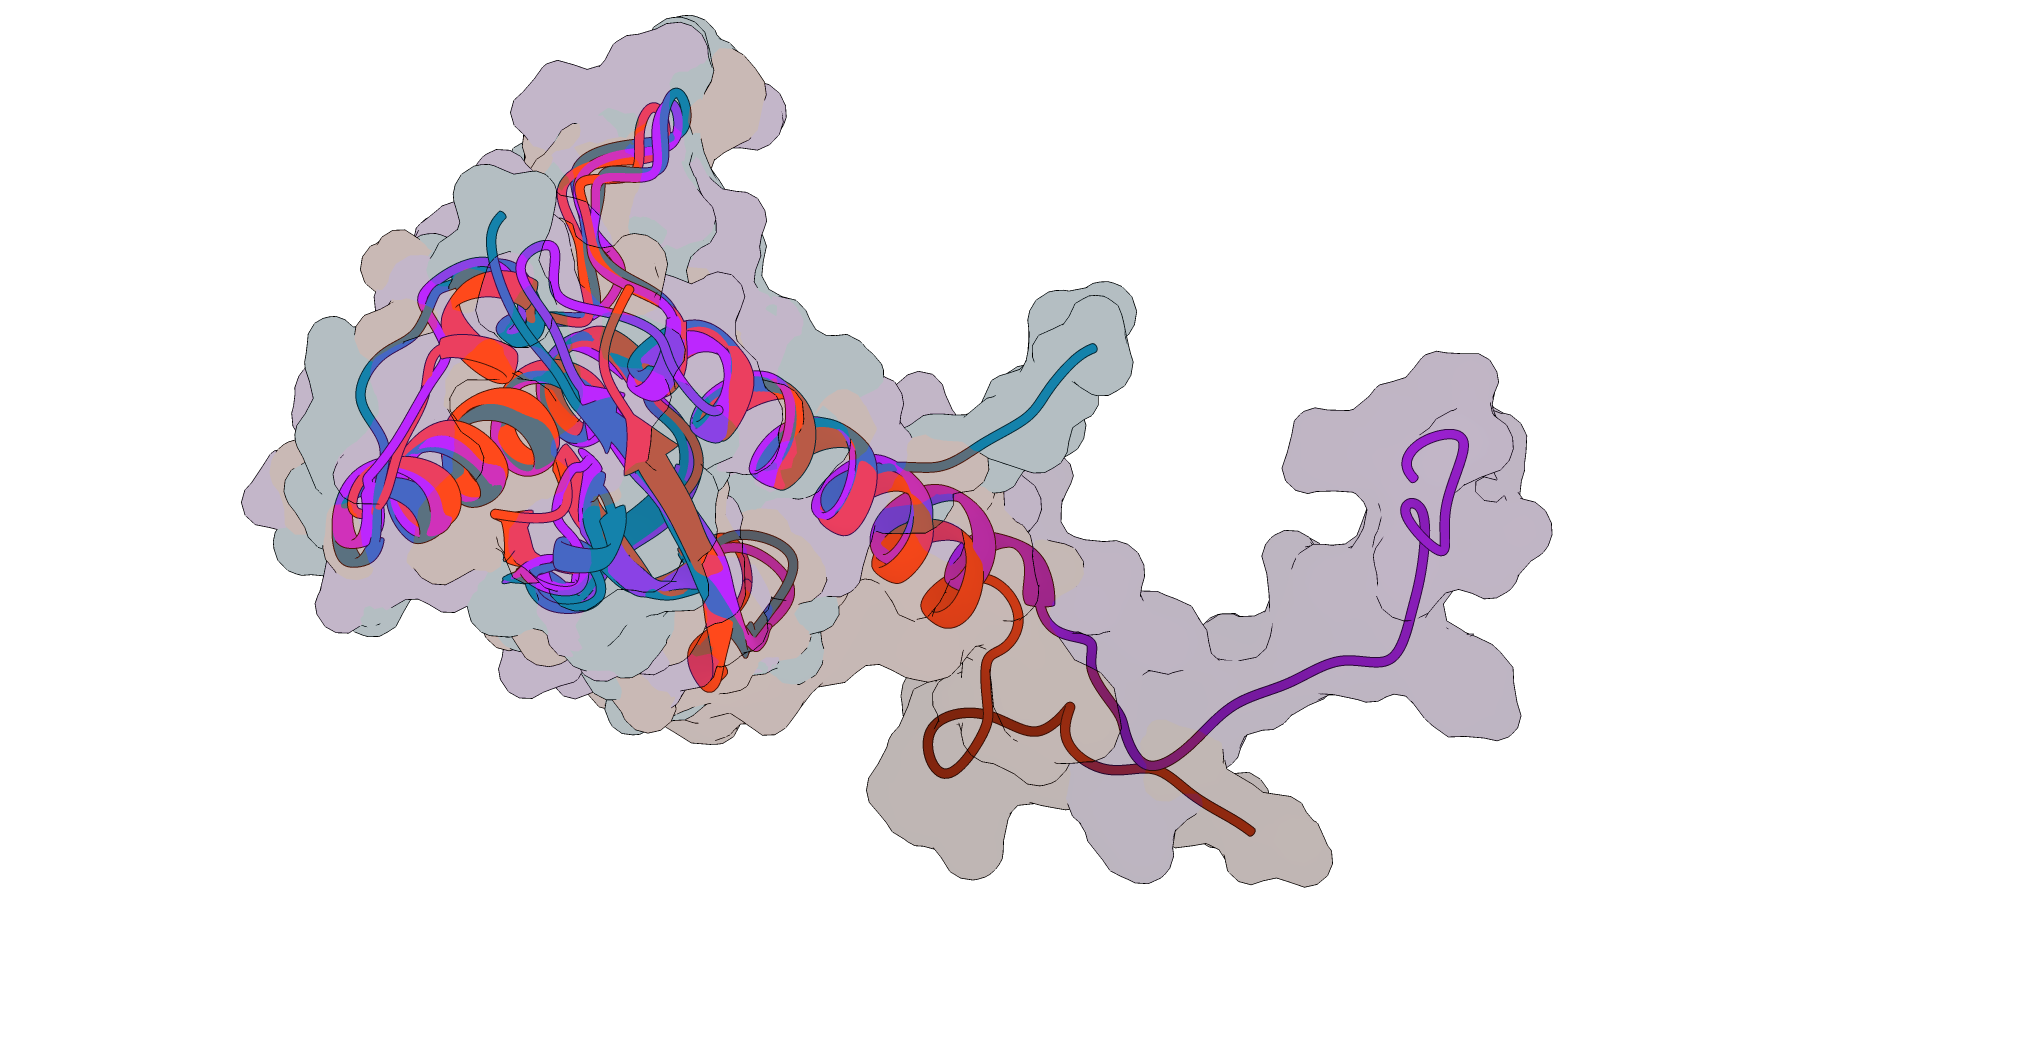
\includegraphics[width=0.8\textwidth, trim={50 10 60 0}, clip]{/Users/joehealey/Documents/Warwick/PhD/Thesis/chapters/chapter3/img/PVC9_gp25.png}
\captionsetup{singlelinecheck=off, justification=justified, font=footnotesize, aboveskip=10pt}
\caption[PVC9 as a tube initiator candidate]{\textsc{\normalsize PVC9 compared to a putative lysozyme and tube initiator.}\vspace{0.1cm} \newline PVC9 (purple), structurally compared to PDB ID 2IA7, a putative lysozyme (blue), and the T4 tube initiator protein gp25 (orange). Based on their structure similarity, PVC9 is likely a tube initiator protein, and this was not previously identified due to a spurious annotation of lysozyme on the better sequence match for PDB 2IA7.}
	\label{initiator}
\end{figure}


Since the role of a tube initiator protein is relevant to the structure and assembly of all caudate structures (as far as is known presently), and no other compelling candidates have been identified so far, PVC9 is therefore likely fulfilling this role. The descriptor ascribed to the PDB ID 2IA7 of a putative lysozyme is almost certainly incorrect.

PVC10 has been another enigmatic protein for some time and still recruits matches to a number of different potential orthologues including proteins such as RNA polymerase subunits and Amyloid proteins. In just a couple of cases when querying the various PVC orthologues of this protein, homology was noted to ``PAAR"-repeat motif proteins. ``PAAR", or Proline-Alanine-Alanine-Repeat proteins are integral components of most caudate structures studied to date, but are extremely variable and difficult to detect. The T6SS alone employs a bewildering diversity of these proteins \citep{Shneider2013}. Inspecting the sequences, there are few repeats to speak of when analysed by RADAR, and none of the orthologues even contain the PAAR subsequence.

PAAR-repeat proteins sit at the apex of the extended $\beta$-prism of the spike complex, sharpening the otherwise slightly blunt face, down to a single atom's diameter potentially. \cite{Schneider2013} describe PAAR proteins in the case of model PDB ID 4JIV as being comprised of nine short $\beta$ strands, 3 of which form a base interacting with the rest of the spike complex following the $\beta$-prism conformation, and the remainder forming $\beta$ hairpins of different length.

The simulated models obtained are fairly poor facsimiles of \emph{bona fide} PAAR proteins of resolved structure, however, all of the models share some characteristics which support the hypothesis. The majority of models adopted a $\beta$-sheet dominated structure, which run head to tail, reminiscent of the $\beta$-prism conformation seen at the base of PAAR protein spikes, suggesting they augment the prism, if not form the spike itself. As these proteins are slightly longer than canonical PAAR proteins, it may be the case that they incorporate more of the $\beta$-prism in to the spike itself, which could account for the slightly shorter prisms seen in the PVC8 models, even taking in to consideration limitations in the simulation quality. This gives the models a similar triangular cross section to the PAAR proteins. Where the structures are not $\beta$-stranded they produce turn regions, which would provide the alternating strand-turn-strand conformation needed to enable $\beta$-hairpins like those seen in the resolved structures. These proteins possibly present a limitation for the simulation software, lacking good tertiary structure models and therefore resorting to largely molecular dynamics based approaches, which has given an energy minimised `collapsed' structure. \vref{PAAR} shows examples of homologous structures and indicative examples of the obtained models.

ADD PAAR IMAGE


\subsubsection{The operon core}
\begin{figure}[h!]
\thisfloatpagestyle{IHA-fancy-style}
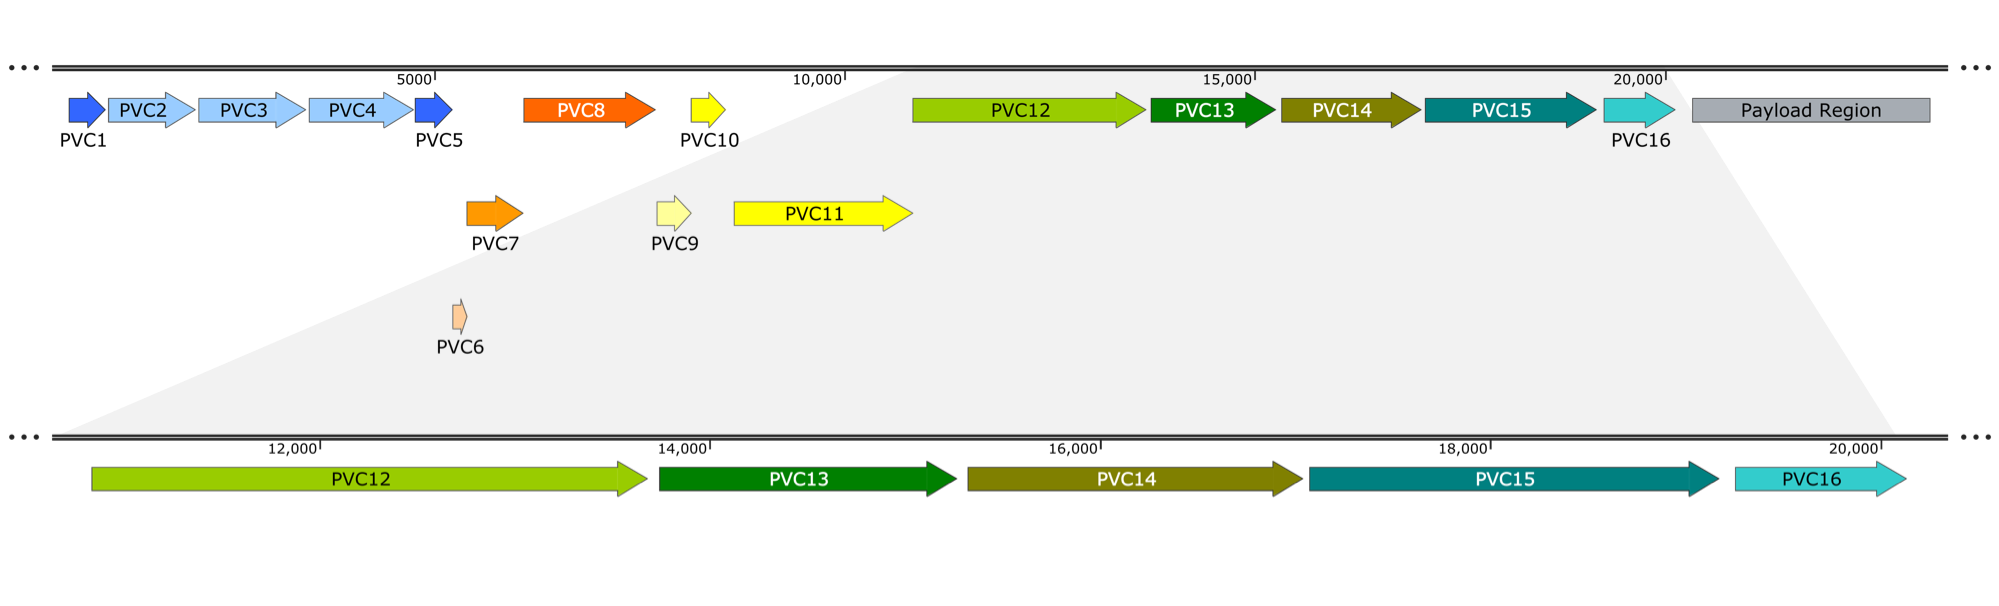
\includegraphics[width=\linewidth]{/Users/joehealey/Documents/Warwick/PhD/Thesis/chapters/chapter3/img/PVC12-16_expanded_map.png}
	\captionsetup{singlelinecheck=off, justification=justified, font=footnotesize, aboveskip=10pt}
	\caption[`Core' protein region of a PVC operon]{\textsc{\normalsize The 5 loci comprising the `core' of a PVC operon with various functions.}\vspace{0.1cm} \newline The Pnf operon is used as an exemplar of the numbering of loci within an archetypal PVC operon, and 3 colourings are used to demarcate the `functional units' of an operon: blue - tube proteins, orange/yellow - spike complex proteins, green/cyan - the operon `core'. The 6 loci that give rise to the operon core are blown up below as an aid to understanding the operon organisation and the proteins under discussion. The `core' is a collection of conserved proteins present in almost all PVC operons, typically comprised of larger, single copy genes, some which are proposed to be structural, but also the proteins responsible for cell surface adhesion, and an ATPase which potentially loads payloads or recycles the tube apparatus.}
	\label{PVC11-16map}
\end{figure}
Tail fibres - highlight hyper variable domains

Tape measure proteins - high in helix? (add the calculations from the hhpred hits).
Tape measure proteins - annotate the MSA with helical regions according to DSSP?
Tape measure proteins - speculate on length


\section{Discussion}
PVCs are a hybrid between T4 and pyocin like structures, with an inner sheath most resembling the former, and an outer sheath the latter.

\addfloat{Summary table of PVC1-16 and their roles}

\clearpage
\small
\rowcolors{2}{gray!10}{white}
\begin{tabularx}{\textwidth}{
>{\raggedright\arraybackslash} m{0.3\textwidth}
>{\raggedright\arraybackslash} X
}
\hiderowcolors
\captionsetup{singlelinecheck=off, justification=justified, font=footnotesize, belowskip=5pt}
\caption[Summary of loci functions in PVC structural biology]{\textsc{\normalsize Summary of putative loci functions for PVC structural proteins.}\vspace{0.1cm} \newline A summary of the proposed primary roles for PVC structural loci. Loci with asterisks indicate new functions proposed as a result of this work.}\\
\label{tubehomologs}\\
Locus & Proposed structure/role in the PVC \\
\hline\hline
\showrowcolors
\hline

PVC1 & Inner tube   \\
PVC2 & Outer sheath   \\
PVC3 & Outer sheath (frequently deleted)   \\
PVC4 & Outer sheath   \\
PVC5* & Possible collar adapter  \\
PVC6 & Unknown (augment/lynchpin?)   \\
PVC7 & Unknown (Possible enzyme/chaperone?)   \\
PVC8 & Spike trimer   \\
PVC9* & Tube initiator   \\
PVC10* & PAAR-like spike augment   \\
PVC11 & Major baseplate protein   \\
PVC12 & Unknown   \\
PVC13 & Host binding tail-fibre chimeras   \\
PVC14 &* Tube `tape measure protein'   \\
PVC15 & Loading/Assembly ATPase   \\
PVC16 &* Tube terminator (?)   \\
\end{tabularx}
\normalsize

It is also interesting that the inner and outer tube orthologies do not share the same provenance. It might be expected that they should all match to the next closest structure (e.g. all matching to the \emph{P. aeruginosa} R-type pyocin). This indicates that the inner and outer sheaths may be subject to different evolutionary pressures. Additionally, interior sheath proteins are smaller and better conserved. This may, therefore, be indicative of \emph{Photorhabdus} honing the exterior of the sheath in different environments. An appealing hypothesis, especially since legacy data has shown that different PVCs are deployed in very particular inducing conditions\todo{move to discussion?}.

Hypotheses for paralogy:
 - Stoichiometry (certainly plausible and may be true in addition to other factors (but why then, are there 3 outer proteins in most operons)).
 - Patchwork idea, or alternating stacks (bar magnets)


PVC5 different exterior charge, because not in main tube! not interacting with PVC2-4!

Differences in R-type pyocin sequence and structure versus other structures may be accounted for by originating from different phage. E.g if PVCs came from T4 and T6SS ancestors, but the R-type Pyocin is known to have come from phage P2 \citep{Nakayama2000}.


Asymbiotica strains ditching an immunogenic outer sheath protein?!

\cite{Hurst2004} demonstrated that Afp2 is required for formation of a toxic Afp. In several PVC operons a deletion in one of the 3 proteins which match to outer sheaths are observed. Initially, it was not obvious which of these 3 proteins, assumed to be equally paralogous, would be deleted in each case. It seemed unusual that 3 outer sheath CDSs would be required whilst only 2 inner sheath CDSs are ever present, if stoichiometry was the only explanation for their paralogy. On further inspection, it appears that the deletions in these outer sheath proteins is always PVC3 rather than 2 or 4. Unpublished communication from the Hurst lab has proposed that PVC4 may actually be a slightly modified variant of the outer tube. This may be such that it functions as an adapter protein at one end of the tube, possibly as a collar that interfaces with the baseplate.

Main remaining mysteries:
PVC6,7,11,12

Basis of 3 copies of the outer sheath. Inner sheath may now have a plausible answer.

Suggest that VgrGs may be somewhat adapted/evolved based on host
Evaluations/Considerations:
Obviously the simulations presented in this chapter are of assorted qualities, and care must be taken when concluding anything from theoretical data alone, however, there is a sufficient body of related proteins for many PVC loci, that comparative modelling can provide, and has provided, hypotheses and potential answers for a number of questions which are not answerable without resolving the structures either experimentally or otherwise.

Template based methods may actually not be ideal - overfitting? If the sequences are similar, but other factors come in to play when folded and thus the structures are not 100\% identical, threading tools would coerce them to fit the `wrong' template.

\subsection{Future work}
Mention PVC6/7 as a deletion candidate
Mention PVC15 as a deletion candidate
 - Involved in assembly in Hursts work.
 - if deleted, do PVCs still assemble, but empty?




